\documentclass[a4paper,12pt,twoside]{memoir}

% Castellano
\usepackage[spanish,es-tabla]{babel}
\selectlanguage{spanish}
\usepackage[utf8]{inputenc}
\usepackage[T1]{fontenc}
\usepackage{lmodern} % scalable font
\usepackage{microtype}
\usepackage{placeins}

\RequirePackage{booktabs}
\RequirePackage[table]{xcolor}
\RequirePackage{xtab}
\RequirePackage{multirow}

% Links
\PassOptionsToPackage{hyphens}{url}\usepackage[colorlinks]{hyperref}
\hypersetup{
	allcolors = {red}
}

% Ecuaciones
\usepackage{amsmath}

% Rutas de fichero / paquete
\newcommand{\ruta}[1]{{\sffamily #1}}

% Párrafos
\nonzeroparskip

% Huérfanas y viudas
\widowpenalty100000
\clubpenalty100000

% Evitar solapes en el header
\nouppercaseheads

% Imagenes
\usepackage{graphicx}
\newcommand{\imagen}[2]{
	\begin{figure}[!h]
		\centering
		\includegraphics[width=0.9\textwidth]{#1}
		\caption{#2}\label{fig:#1}
	\end{figure}
	\FloatBarrier
}

\newcommand{\imagenflotante}[2]{
	\begin{figure}%[!h]
		\centering
		\includegraphics[width=0.9\textwidth]{#1}
		\caption{#2}\label{fig:#1}
	\end{figure}
}



% El comando \figura nos permite insertar figuras comodamente, y utilizando
% siempre el mismo formato. Los parametros son:
% 1 -> Porcentaje del ancho de página que ocupará la figura (de 0 a 1)
% 2 --> Fichero de la imagen
% 3 --> Texto a pie de imagen
% 4 --> Etiqueta (label) para referencias
% 5 --> Opciones que queramos pasarle al \includegraphics
% 6 --> Opciones de posicionamiento a pasarle a \begin{figure}
\newcommand{\figuraConPosicion}[6]{%
  \setlength{\anchoFloat}{#1\textwidth}%
  \addtolength{\anchoFloat}{-4\fboxsep}%
  \setlength{\anchoFigura}{\anchoFloat}%
  \begin{figure}[#6]
    \begin{center}%
      \Ovalbox{%
        \begin{minipage}{\anchoFloat}%
          \begin{center}%
            \includegraphics[width=\anchoFigura,#5]{#2}%
            \caption{#3}%
            \label{#4}%
          \end{center}%
        \end{minipage}
      }%
    \end{center}%
  \end{figure}%
}

%
% Comando para incluir imágenes en formato apaisado (sin marco).
\newcommand{\figuraApaisadaSinMarco}[5]{%
  \begin{figure}%
    \begin{center}%
    \includegraphics[angle=90,height=#1\textheight,#5]{#2}%
    \caption{#3}%
    \label{#4}%
    \end{center}%
  \end{figure}%
}
% Para las tablas
\newcommand{\otoprule}{\midrule [\heavyrulewidth]}
%
% Nuevo comando para tablas pequeñas (menos de una página).
\newcommand{\tablaSmall}[5]{%
 \begin{table}
  \begin{center}
   \rowcolors {2}{gray!35}{}
   \begin{tabular}{#2}
    \toprule
    #4
    \otoprule
    #5
    \bottomrule
   \end{tabular}
   \caption{#1}
   \label{tabla:#3}
  \end{center}
 \end{table}
}

%
%Para el float H de tablaSmallSinColores
\usepackage{float}

%
% Nuevo comando para tablas pequeñas (menos de una página).
\newcommand{\tablaSmallSinColores}[5]{%
 \begin{table}[H]
  \begin{center}
   \begin{tabular}{#2}
    \toprule
    #4
    \otoprule
    #5
    \bottomrule
   \end{tabular}
   \caption{#1}
   \label{tabla:#3}
  \end{center}
 \end{table}
}

\newcommand{\tablaApaisadaSmall}[5]{%
\begin{landscape}
  \begin{table}
   \begin{center}
    \rowcolors {2}{gray!35}{}
    \begin{tabular}{#2}
     \toprule
     #4
     \otoprule
     #5
     \bottomrule
    \end{tabular}
    \caption{#1}
    \label{tabla:#3}
   \end{center}
  \end{table}
\end{landscape}
}

%
% Nuevo comando para tablas grandes con cabecera y filas alternas coloreadas en gris.
\newcommand{\tabla}[6]{%
  \begin{center}
    \tablefirsthead{
      \toprule
      #5
      \otoprule
    }
    \tablehead{
      \multicolumn{#3}{l}{\small\sl continúa desde la página anterior}\\
      \toprule
      #5
      \otoprule
    }
    \tabletail{
      \hline
      \multicolumn{#3}{r}{\small\sl continúa en la página siguiente}\\
    }
    \tablelasttail{
      \hline
    }
    \bottomcaption{#1}
    \rowcolors {2}{gray!35}{}
    \begin{xtabular}{#2}
      #6
      \bottomrule
    \end{xtabular}
    \label{tabla:#4}
  \end{center}
}

%
% Nuevo comando para tablas grandes con cabecera.
\newcommand{\tablaSinColores}[6]{%
  \begin{center}
    \tablefirsthead{
      \toprule
      #5
      \otoprule
    }
    \tablehead{
      \multicolumn{#3}{l}{\small\sl continúa desde la página anterior}\\
      \toprule
      #5
      \otoprule
    }
    \tabletail{
      \hline
      \multicolumn{#3}{r}{\small\sl continúa en la página siguiente}\\
    }
    \tablelasttail{
      \hline
    }
    \bottomcaption{#1}
    \begin{xtabular}{#2}
      #6
      \bottomrule
    \end{xtabular}
    \label{tabla:#4}
  \end{center}
}

%
% Nuevo comando para tablas grandes sin cabecera.
\newcommand{\tablaSinCabecera}[5]{%
  \begin{center}
    \tablefirsthead{
      \toprule
    }
    \tablehead{
      \multicolumn{#3}{l}{\small\sl continúa desde la página anterior}\\
      \hline
    }
    \tabletail{
      \hline
      \multicolumn{#3}{r}{\small\sl continúa en la página siguiente}\\
    }
    \tablelasttail{
      \hline
    }
    \bottomcaption{#1}
  \begin{xtabular}{#2}
    #5
   \bottomrule
  \end{xtabular}
  \label{tabla:#4}
  \end{center}
}



\definecolor{cgoLight}{HTML}{EEEEEE}
\definecolor{cgoExtralight}{HTML}{FFFFFF}

%
% Nuevo comando para tablas grandes sin cabecera.
\newcommand{\tablaSinCabeceraConBandas}[5]{%
  \begin{center}
    \tablefirsthead{
      \toprule
    }
    \tablehead{
      \multicolumn{#3}{l}{\small\sl continúa desde la página anterior}\\
      \hline
    }
    \tabletail{
      \hline
      \multicolumn{#3}{r}{\small\sl continúa en la página siguiente}\\
    }
    \tablelasttail{
      \hline
    }
    \bottomcaption{#1}
    \rowcolors[]{1}{cgoExtralight}{cgoLight}

  \begin{xtabular}{#2}
    #5
   \bottomrule
  \end{xtabular}
  \label{tabla:#4}
  \end{center}
}




\graphicspath{ {./img/} }

% Capítulos
\chapterstyle{bianchi}
\newcommand{\capitulo}[2]{
	\setcounter{chapter}{#1}
	\setcounter{section}{0}
	\setcounter{figure}{0}
	\setcounter{table}{0}
	\chapter*{#2}
	\addcontentsline{toc}{chapter}{#2}
	\markboth{#2}{#2}
}

% Apéndices
\renewcommand{\appendixname}{Apéndice}
\renewcommand*\cftappendixname{\appendixname}

\newcommand{\apendice}[1]{
	%\renewcommand{\thechapter}{A}
	\chapter{#1}
}

\renewcommand*\cftappendixname{\appendixname\ }

% Formato de portada
\makeatletter
\usepackage{xcolor}
\newcommand{\tutor}[1]{\def\@tutor{#1}}
\newcommand{\course}[1]{\def\@course{#1}}
\definecolor{cpardoBox}{HTML}{E6E6FF}
\def\maketitle{
  \null
  \thispagestyle{empty}
  % Cabecera ----------------
\noindent
\includegraphics[width=\textwidth]{cabecera}\vspace{1cm}%
  \vfill
  % Título proyecto y escudo informática ----------------
  \colorbox{cpardoBox}{%
    \begin{minipage}{.8\textwidth}
      \vspace{.5cm}\Large
      \begin{center}
      \textbf{TFG del Grado en Ingeniería Informática}\vspace{.6cm}\\
      \textbf{\LARGE\@title{}}
      \end{center}
      \vspace{.2cm}
    \end{minipage}

  }%
  \hfill\begin{minipage}{.20\textwidth}
    
\includegraphics[width=\textwidth]{escudoInfor}
  \end{minipage}
  \vfill
  % Datos de alumno, curso y tutores ------------------
  \begin{center}%
  {%
    \noindent\LARGE
    Presentado por \@author{}\\ 
    en Universidad de Burgos --- \@date{}\\
    Tutor: \@tutor{}\\
  }%
  \end{center}%
  \null
  \cleardoublepage
  }
\makeatother


% Datos de portada
\title{título del TFG \\Documentación Técnica}
\author{nombre alumno}
\tutor{nombre tutor}
\date{\today}

\begin{document}

\maketitle



\cleardoublepage



%%%%%%%%%%%%%%%%%%%%%%%%%%%%%%%%%%%%%%%%%%%%%%%%%%%%%%%%%%%%%%%%%%%%%%%%%%%%%%%%%%%%%%%%



\frontmatter


\clearpage

% Indices
\tableofcontents

\clearpage

\listoffigures

\clearpage

\listoftables

\clearpage

\mainmatter

\appendix

\apendice{Plan de Proyecto Software}

\section{Introducción}\label{plan-proyecto-introduccion}

La fase de planificación es esencial en cualquier proyecto. Durante esta etapa, se calculan el trabajo, el tiempo y el dinero necesarios para completar el proyecto. Para ello, se analiza detalladamente cada una de las partes que lo componen, lo que permite conocer los recursos necesarios para su realización. En este anexo se describe todo este proceso.

La fase de planificación se puede dividir en dos partes:

\begin{itemize}
  \item \textbf{La planificación temporal:} se crea un calendario o cronograma. Aquí se calcula el tiempo necesario para completar cada una de las partes del proyecto. Se debe establecer una fecha de inicio fija y una fecha de finalización estimada, considerando la importancia de cada tarea y los requisitos necesarios para comenzar a trabajar en ellas.
  \item \textbf{El estudio de viabilidad:} se enfoca en la factibilidad del proyecto y se divide en dos apartados. 
  \begin{itemize}
    \item \textbf{La viabilidad económica:} en esta parte se estiman los costos y los beneficios que podría traer la realización del proyecto. 
    \item \textbf{La viabilidad legal:} aquí es donde se tiene en cuenta el contexto del proyecto y toca aquella ley que le afecta. Se deben analizar todas aquellas que afecten al proyecto.
  \end{itemize}
\end{itemize}

\section{Planificación temporal}\label{planificacion-temporal}

En líneas generales, se ha seguido la metodología Scrum, aunque de manera adaptada a la situación de ser el único desarrollador, manteniendo ciertos principios clave.

\begin{itemize}
  \item Se aplicó una estrategia de desarrollo incremental mediante iteraciones (sprints) y revisiones.
  \item La duración media de los sprints ha sido de dos semanas.
  \item Aunque no se han tenido reuniones diarias, se han realizado revisiones periódicas al final de cada sprint para evaluar el progreso y planificar el siguiente.
  \item Esto ha permitido mantener la esencia de la mejora continua y la entrega incremental de valor.
\end{itemize}

Cabe mencionar que no fue hasta la reunión de control del 26 de marzo cuando se empezó a reflejar el progreso en GitHub, añadiendo todas las issues de reuniones anteriores y etiquetándolas con S1, S2 y S3 en el nombre para indicar la semana correspondiente. Por ello, en GitHub todas las issues aparecen como añadidas entre el 26 y el 28 de marzo. Zube se comenzó a utilizar para organizar mejor los sprints a partir del sprint 4, debido a la recomendación de Carlos para tener un mejor control de estos.

\subsection{Sprint 0 (04/03/2024 - 11/03/2024)}\label{sprint-0}

La reunión que dio inicio a este sprint marcó el comienzo del proyecto de fin de carrera. Inicialmente, Pedro Latorre había explicado en qué consistía la idea inicial del proyecto en una reunión previa. En esta ocasión, se profundizó más en la idea y se indicaron unas pautas a seguir para investigar el estado del arte en esta área y plantear unos objetivos a cumplir durante este primer sprint.

Los objetivos de la reunión del primer sprint fueron: crear un repositorio en GitHub para el proyecto, probar dos métodos de procesamiento de imágenes, específicamente el Análisis de Componentes Principales (PCA) y la Teoría Retinex, y guardar la imagen resultante permitiendo acceder al valor de cada píxel. También se acordó investigar y aplicar métodos de agrupamiento de datos, como K-Means, en la imagen original y en la imagen procesada para comparar los resultados.

Además, se decidió eliminar el cuarto canal en las imágenes que lo tuvieran y evaluar críticamente los resultados obtenidos. Se enfatizó que no se esperaran resultados inmediatos, sino que se debía evaluar y descartar posibles caminos de manera progresiva.

En este momento del proyecto, simplemente se crearon una serie de tareas a completar antes de la próxima semana, por lo que no se tiene un registro temporal en Zube de cuándo se completó cada tarea. Más tarde, estas tareas se pasaron a GitHub el 26/03/2024 por recomendación del tutor, ya que así se podía reflejar el trabajo realizado hasta el momento. Estas issues tienen en el nombre [S1].

\subsection{Sprint 1 (11/03/2024 - 25/03/2024)}\label{sprint-1}

Este sprint tuvo como objetivos: mostrar la representación del histograma de los valores de los píxeles de cada canal en la imagen resultante, determinar los valores mínimos y máximos de los píxeles, y visualizar la matriz resultante utilizando imshow. Se discutió que, aunque imshow(M, []) normaliza la imagen para visualización, imwrite guarda la imagen sin normalizar. Se acordó guardar la imagen utilizando el método saveas para conservar el rango dinámico y almacenar la matriz en un archivo .mat con el resultado de la transformación. También se destacó la importancia de guardar una imagen que se pueda visualizar fácilmente y familiarizarse con los resultados de cada método aplicado.

Se decidió añadir los métodos de agrupamiento FUZZY C-Means y GMM, y probar otros métodos de agrupamiento que tengan en cuenta el contexto y no solo el valor del píxel. Además, se acordó buscar información sobre Geoffrey Machlachlan para profundizar en el tema.

Al igual que en el sprint 0, simplemente se crearon una serie de tareas a completar antes de la próxima semana, por lo que no se tiene un registro temporal en Zube y en GitHub. Las tareas fueron añadidas el 26/03/2024. Estas issues tienen en el nombre [S2].

\subsection{Sprint 2 (25/03/2024 - 04/04/2024)}\label{sprint-2}

Este sprint tuvo como objetivo: trasladar los algoritmos de agrupamiento de Python a MATLAB, ya que los tiempos de ejecución en Python, el lenguaje utilizado hasta ese momento, eran muy elevados. Se decidió crear una comparación en la misma ventana, dependiendo del número de centros, para así poder observar las diferencias de manera más cómoda y rápida. Además, se acordó agregar 4-5 métodos más de transformación invariante.

También se decidió generar la imagen ground truth y evaluar el resultado mediante una máscara binaria, calculando la tasa de acierto con la fórmula  (nº de píxeles que coinciden / nº total de píxeles) * 100, y mostrar en la ventana el valor de esta tasa.

Al igual que en el sprint 0 y sprint 1, simplemente se crearon una serie de tareas a completar antes de la próxima semana, por lo que no se tiene un registro temporal en Zube. En GitHub, las tareas fueron añadidas el 26/03/2024. Estas issues tienen en el nombre [S3].

\subsection{Sprint 3 (04/04/2024 - 18/04/2024)}\label{sprint-3}

En la reunión de preparación de este sprint, Carlos López se unió como cotutor al proyecto a solicitud de Pedro Latorre. En el futuro, Carlos López pasaría a ser el tutor del proyecto de fin de grado.

Este sprint tuvo como objetivo familiarizarse con Overleaf y comenzar a rellenar los tres primeros apartados del documento. Además, se acordó crear una cuenta en Zube para organizar las tareas en milestones y reorganizar los directorios del proyecto. La nueva estructura incluirá un directorio "doc" con la plantilla de Ubuvirtual y un directorio para el programa MATLAB, que contendrá todos los métodos utilizados, separados en distintos scripts para mejorar la modularidad, reutilización y mantenibilidad del código.

Otro objetivo fue la integración de MATLAB con una aplicación web, iniciando un pequeño proyecto en GitHub para gestionar esta integración. También se planteó el desarrollo de una pequeña aplicación de escritorio de MATLAB, que servirá para probar distintos algoritmos sobre diferentes imágenes. De esta manera, además de demostrar numéricamente que hay una mejora notable tras la aplicación de métodos invariantes sobre piezas metálicas, permitirá probar distintos métodos sobre imágenes propias de forma sencilla y visual.

En el sprint anterior, no se logró encontrar un método de agrupamiento con contexto espacial que supusiera una mejora notable en los resultados, por lo que esta issue no se cerrará y formará parte también de este cuarto sprint.

Al ser este el primer sprint en el que se incorporó Zube para gestionar las issues abiertas, aún no se dominaba completamente la herramienta. Aunque ayudó con la gestión, no se creó el sprint en Zube, por lo que no se dispone de un gráfico burndown de este sprint.

\subsection{Sprint 4 (18/04/2024 - 02/05/2024)}\label{sprint-4}

Es en este sprint cuando se comienza a reflejar formalmente los distintos sprints en Zube. Gracias a esto, a partir de este momento, resultó más cómodo trabajar con las issues de cada sprint.

Este sprint tuvo como objetivos: mejorar las funcionalidades de la aplicación y realizar cambios menores en el texto mostrado al usuario dentro de la aplicación para evitar confusiones y corregir incoherencias. Se acordó cambiar el orden en el que se muestran los resultados de la aplicación y se discutió la importancia de eliminar las imágenes mostradas de ejecuciones anteriores.

También se añadió un selector para guardar los archivos y su correspondiente mensaje de confirmación indicando que los archivos se han guardado correctamente. Además, se buscó una solución para el problema relacionado con el sistema de directorios donde se guardan los archivos.

Finalmente, se planteó la creación de otra aplicación para poder probar con imágenes propias. Al tener una imagen ground truth, se podría obtener un porcentaje de acierto de la ejecución, lo que ayudaría a evaluar mejor los resultados obtenidos.

\imagen{sprint4}{Burndown del sprint 4.}

Como se puede ver en el gráfico burndown \ref{fig:sprint4}, las issues de este sprint no fueron marcadas como completadas hasta el último día. En ese momento, no se era consciente de que debían cerrarse en lugar de dejarlas en revisión para cerrarlas después de la reunión.


\subsection{Sprint 5 (02/05/2024 - 23/05/2024)}\label{sprint-5}

Este sprint tuvo como objetivo mejorar la experiencia del usuario y optimizar la funcionalidad de la aplicación. Se implementaron notificaciones periódicas sobre el estado de la ejecución, indicando que podría tomar mucho tiempo, además de añadir la funcionalidad de borrar resultados anteriores. También se realizaron pequeños cambios en la interfaz, como eliminar el "-" de los porcentajes y añadir un botón para guardar imágenes.

Se realizaron distintas modificaciones en la estructura de la interfaz, añadiendo menús de ayuda, una lista de nombres de imágenes en caché, un menú de bienvenida y ayuda contextual. Se actualizó el nombre de los archivos de resultados, añadiendo la fecha de ejecución al inicio. Además, se corrigieron errores en la selección de imágenes desde rutas diferentes a /data y se mejoró la gestión de errores.

Se llegó a la conclusión de agregar una caché de imágenes para almacenar temporalmente los resultados, cargando ejecuciones anteriores con los mismos parámetros para reducir el coste computacional. Al cerrar la aplicación, la caché se borraría. Finalmente, se planteó la corrección de algunos errores detectados en los algoritmos, así como una mejora de la documentación y el README del proyecto.

\imagen{sprint5}{Burndown del sprint 5.}

Como se puede ver en el gráfico burndown \ref{fig:sprint5}, las issues de este sprint no fueron marcadas como completadas hasta el último día. En ese momento, no se era consciente de que debían cerrarse en lugar de dejarlas en revisión para cerrarlas después de la reunión.


\subsection{Sprint 6 (23/05/2024 - 30/05/2024)}\label{sprint-6}

Este sprint tuvo como objetivo mejorar la funcionalidad y usabilidad de la aplicación. Se planean diversas mejoras en la documentación en HTML y la creación de un README en la carpeta de imágenes. Además, se modificará la visualización de los nombres de las imágenes dentro de la aplicación y se añadirán tooltips para una mejor comprensión del usuario.

Se establecerán condiciones numéricas en los campos de número de centros y se añadirá un límite máximo de iteraciones en los métodos de agrupamiento. También se trabajará en la caché para hacerla persistente, permitiendo borrar el historial y mejorando su escalabilidad.

En cuanto a la evaluación de la calidad, se incorporará una medida de comparación utilizando la imagen ground truth y se mejorará la nomenclatura de los algoritmos invariantes, reemplazando los nombres vacíos con “no aplicado”. Se abordarán problemas técnicos como la minimización de la app al cargar una imagen, la eliminación de la imagen ground truth al introducir una nueva que no tenga una asociada, y se revisarán soluciones para evitar que la aplicación se detenga por errores. Además, se tratará de introducir concurrencia para manejar tareas como cancelar la ejecución.

\imagen{sprint6}{Burndown del sprint 6.}

Como se puede ver en el gráfico burndown \ref{fig:sprint6}, las issues de este sprint se fueron cerrando correctamente a medida que se completaban.


\subsection{Sprint 7 (31/05/2024 - 10/06/2024)}\label{sprint-7}

Este sprint tuvo como objetivo preparar la primera release oficial de la aplicación. Se realizarán mejoras en la gestión de errores para asegurar una experiencia de usuario más robusta. Además, se tratará de aplicar concurrencia para permitir la cancelación de la ejecución, una tarea que no se logró completar en el sprint anterior.

Se deshabilitarán los botones durante la ejecución de procesos para evitar acciones no deseadas y se revisará el código, actualizando la documentación interna para mantener la coherencia. También se implementará soporte bilingüe, añadiendo opciones en español e inglés para hacer la aplicación accesible a un público más amplio.

\imagen{sprint7}{Burndown del sprint 7.}

Como se puede ver en el gráfico burndown \ref{fig:sprint7}, las issues de este sprint se fueron cerrando correctamente a medida que se completaban, a excepción de una que, por falta de tiempo, quedó pendiente para completar en el siguiente sprint.


\subsection{Sprint 8 (11/06/2024 - 27/06/2024)}\label{sprint-8}

En este sprint, se implementaron mejoras y se preparó la aplicación para su versión oficial. Se mejoraron los tooltips, especialmente el de centros, y se añadió la opción de imprimir y visualizar imágenes en la caché, además de modificar el botón "Abrir directorio" por "Ver imágenes". Se habilitó la ordenación por filas en la caché y se actualizó la imagen de bienvenida.

Para garantizar compatibilidad, la aplicación se adaptó a Linux y Mac, y se realizaron pruebas unitarias. Se creó un README detallado y se reorganizaron los directorios, eliminando los obsoletos. También se subió la versión anterior con mejoras en el manejo de errores y adaptación al inglés.

En la documentación, se añadieron citas y se revisaron correcciones en la memoria, y se redactaron el plan de proyecto, especificaciones de requisitos y diseño en los anexos.

Finalmente, se realizó la versión con todos los cambios del sprint, consolidando las mejoras para la versión final.

\imagen{sprint8}{Burndown del sprint 8.}

Como se puede apreciar en la figura \ref{fig:sprint8}, no se lograron finalizar todas las tareas planificadas para este supuesto sprint final, debido a que la documentación requirió una considerable cantidad de tiempo. Por este motivo, se acordó reunirse a mitad de semana con todas estas tareas finalizadas y con al menos una versión inicial de la documentación completada.

\subsection{Sprint 9 (28/06/2024 - 01/07/2024)}\label{sprint-9}

Este sprint se dedicó completamente a finalizar las tareas pendientes del periodo anterior, incluyendo la elaboración de una primera versión de la documentación, tanto de la memoria como de los anexos. Además, se identificó y resolvió un error en la aplicación.

\subsection{Resumen del tiempo empleado}\label{resumen-del-tiempo-empleado}

A continuación se muestra un resumen del tiempo dedicado a la realización del proyecto.

\begin{table}[h!]
    \centering
    \begin{tabular}{l l}
        \hline
        \textbf{Categoría}      & \textbf{Tiempo (h)} \\
        \hline
        \textbf{Sprint 0}       & 20    \\
        \textbf{Sprint 1}       & 32    \\
        \textbf{Sprint 2}       & 20    \\
        \textbf{Sprint 3}       & 26    \\
        \textbf{Sprint 4}       & 49    \\
        \textbf{Sprint 5}       & 54    \\
        \textbf{Sprint 6}       & 28    \\
        \textbf{Sprint 7}       & 42    \\
        \textbf{Sprint 8}       & 71    \\
        \textbf{Sprint 9}       & 22    \\
        \hline
        \textbf{Total}          & \textbf{364}\\
        \hline
    \end{tabular}
    \caption{Desglose de tiempo dedicado al proyecto.}\label{tabla:tiempo-dedicado-al-proyecto}
\end{table}

\section{Estudio de viabilidad}\label{estudio-de-viabilidad}

A continuación, se realizará tanto el estudio de viabilidad económica como el de viabilidad legal.

\subsection{Viabilidad económica}\label{viabilidad-economica}

En este apartado se analizarán los costes y beneficios estimados de haber desarrollado el proyecto en un entorno empresarial. Cabe mencionar que dichos datos son aproximados.

\subsubsection{Costes}\label{costes}

A continuación, se realizará tanto el análisis de costes materiales y beneficios.

\textbf{Costes materiales:}

En este apartado se desglosarán todos aquellos costes materiales, tanto de hardware como de software, necesarios para el correcto desarrollo del proyecto. En ambos casos, se considera que se amortizarán a 5 años y se han utilizado durante los cuatro meses de desarrollo del proyecto.

El desglose de todos los dispositivos hardware necesarios para la realización del proyecto se encuentra a continuación en la figura \ref{tabla:costes-de-hardware}.

\begin{table}[h!]
    \centering
    \begin{tabular}{l l l}
        \hline
        \textbf{Concepto}               & \textbf{Coste}    & \textbf{Coste amortizado} \\
        \hline
        \textbf{Ordenador portátil}     & 900,00€           & 60,00€                    \\
        \hline
        \textbf{Total}                  & \textbf{900,00€}  & \textbf{60,00€}           \\
        \hline
    \end{tabular}
    \caption{Costes de hardware.}\label{tabla:costes-de-hardware}
\end{table}

En cuanto a las licencias software no gratuitas se tiene el siguiente desglose en la figura \ref{tabla:costes-de-software}.

\begin{table}[h!]
    \centering
    \begin{tabular}{l l l}
        \hline
        \textbf{Concepto}                   & \textbf{Coste}        & \textbf{Coste amortizado} \\
        \hline
        \textbf{Windows 10 Pro}             & 259,00€               & 17,27€                    \\
        \textbf{MATLAB Academic (Anual)}    & 262,00€               & 87,33€                    \\
        \hline
        \textbf{Total}                      & \textbf{521,00€}      & \textbf{104,60€}          \\
        \hline
    \end{tabular}
    \caption{Costes de software.}\label{tabla:costes-de-software}
\end{table}

Hay que destacar que la licencia de MATLAB utilizada ha sido la Academic que la propia Universidad de Burgos ofrece a los alumnos, la cual se paga anualmente.

\textbf{Costes de personal:}

El proyecto lo ha llevado a cabo un ingeniero informático recién graduado a tiempo completo durante cuatro meses. Se considera que el salario bruto anual es de 24.000,00€ \cite{sueldoIIespaña}, el IRPF sobre el salario bruto es del 13,55\% y la Seguridad Social es del 6,35\% respectivamente como se puede ver en la figura \ref{tabla:costes-de-personal}.

\begin{table}[h!]
    \centering
    \begin{tabular}{l l}
        \hline
        \textbf{Concepto}                   & \textbf{Coste}        \\
        \hline
        \textbf{Salario anual en bruto}     & 24.000,00€            \\
        \textbf{IRPF}                       & 3.251,04€             \\
        \textbf{Seguridad Social}           & 1.524,00€             \\
        \textbf{Salario anual neto}         & 19.224,96€            \\
        \hline
        \textbf{Total 4 meses}              & \textbf{8.000,00€}    \\
        \hline
    \end{tabular}
    \caption{Costes de personal.}\label{tabla:costes-de-personal}
\end{table}

\textbf{Costes totales:}

El sumatorio de todos los distintos tipos de costes se encuentra en la figura \ref{tabla:costes-de-totales}.

\begin{table}[h!]
    \centering
    \begin{tabular}{l l}
        \hline
        \textbf{Concepto}   & \textbf{Coste}        \\
        \hline
        \textbf{Hardware}   & 60,00€                \\
        \textbf{Software}   & 104,60€               \\
        \textbf{Personal}   & 8.000,00€             \\
        \hline
        \textbf{Total}      & \textbf{8.164,60€}    \\
        \hline
    \end{tabular}
    \caption{Costes totales.}\label{tabla:costes-de-totales}
\end{table}

\subsubsection{Beneficios}\label{beneficios}

La aplicación desarrollada se distribuirá de forma libre y sin restricciones, permitiendo su uso sin limitaciones adicionales. La única condición necesaria para su funcionamiento será disponer de MATLAB. En una fase posterior, se evaluará la posibilidad de incorporar características adicionales que mejoren la experiencia del usuario, manteniendo siempre el enfoque en la accesibilidad y la libertad de uso.

\subsection{Viabilidad legal}\label{viabilidad-legal}

Apartado dedicado al marco legal que envuelve el proceso de desarrollo del proyecto, su distribución, modificación y utilización. No es necesario atender al uso de licencias de terceros, pues todo el proyecto ha sido desarrollado con la licencia MATLAB Academic proporcionada por la Universidad de Burgos para desarrolladores individuales o estudiantes y bajo una finalidad no comercial. En concreto, la licencia utilizada ha sido:

\begin{itemize}
  \item \textbf{MATLAB Academic:} Al tratarse de un desarrollador individual, el uso de la licencia MATLAB Academic está justificado. Esta licencia es distribuida de forma gratuita por la Universidad de Burgos a sus alumnos.
\end{itemize}

El proyecto actual ha sido asignado bajo una licencia Creative Commons \cite{cc4}. Esto implica que cualquier usuario es libre de compartir, redistribuir y adaptar la aplicación, siempre y cuando se cumplan las siguientes condiciones:

\begin{itemize}
  \item \textbf{Atribución:} Se debe dar crédito apropiado al autor original, proporcionando un enlace a la licencia e indicando si se han realizado cambios.
  \item \textbf{NoComercial:} No se puede utilizar el material para fines comerciales.
  \item \textbf{CompartirIgual:} Si se remezcla, transforma, o crea a partir del material, se debe distribuir el material modificado bajo la misma licencia que el original.
\end{itemize}

Esta licencia asegura que la aplicación mantenga su accesibilidad y flexibilidad, fomentando la colaboración y el desarrollo comunitario mientras protege los derechos del autor original.

\apendice{Especificación de Requisitos}

\section{Introducción}\label{intoduccion}

Este anexo recoge la especificación de requisitos que define el comportamiento del sistema desarrollado. Se han seguido las recomendaciones del estándar IEEE 830-1998 \cite{ieee}, que establece que una buena especificación de requisitos software debe ser:

\begin{itemize}
    \item \textbf{Completa:} todos los requerimientos deben estar incluidos y todas las referencias definidas.
    \item \textbf{Consistente:} debe ser coherente tanto internamente como con otros documentos de especificación.
    \item \textbf{Inequívoca:} la redacción debe ser clara para evitar malentendidos.
    \item \textbf{Correcta:} el software debe cumplir con los requisitos especificados.
    \item \textbf{Trazable:} debe ser posible rastrear la historia, ubicación o aplicación de un ítem a través de su identificación documentada.
    \item \textbf{Priorizable:} los requisitos deben poder organizarse jerárquicamente según su relevancia para el negocio, clasificándolos en esenciales, condicionales y opcionales.
    \item \textbf{Modificable:} los requerimientos deben ser fácilmente modificables.
    \item \textbf{Verificable:} debe existir un método finito y sin costo para probar los requisitos.
\end{itemize}

\section{Objetivos generales}\label{objetivos-generales}

El proyecto tiene los siguientes objetivos generales.

\begin{itemize}
    \item Demostrar que al aplicar métodos de transformación invariante, se consiguen mejores resultados a la hora de identificar piezas metálicas mediante métodos de segmentación de imágenes.
    \item Desarrollar una aplicación para de escritorio que permita al usuario identificar la pieza de una imagen que introduzca ofreciendo diferentes algoritmos tanto de transformación invariante (propuestos por Álvarez \cite{alvarez2011}, Maddern \cite{maddern2014}, Krajník \cite{krajník2015}, Upcroft \cite{upcroft2014} y PCA \cite{pca2017}) como de segmentación de imágenes (K-Means \cite{MATLAB:2023bKmeans}, Fuzzy C-Means \cite{MATLAB:2023bFuzzy}, GMM \cite{MATLAB:2023bGMM} y segmentación con información espacial \cite{wang2012hmrf}).
    \item Desarrollar una aplicación para de escritorio que permita mostrar la mejoría que suponen los métodos de transformación invariante mostrando una comparación de los resultados tanto visual como numérica.
    \item Guardar los resultados tanto de la imagen original, la resultante del método de transformación invariante como de las correspondientes imágenes tras la segmentación.
\end{itemize}

\section{Catálogo de requisitos}\label{catalogo-de-requisitos}

En este apartado se enumeran los requisitos específicos que se derivan de los objetivos generales del proyecto.

\subsection{Requisitos funcionales}\label{requisitos-funcionales}

\begin{itemize}
    \item \textbf{RF-1 Gestión de transformación invariante:} la aplicación debe ser capaz de gestionar la transformación invariante sobre imágenes.
    \begin{itemize}
        \item \textbf{RF-1.1 Seleccionar imagen:} el usuario debe poder seleccionar una imagen sobre la cual aplicar las diferentes transformaciones.
        \begin{itemize}
            \item \textbf{RF-1.1.1 Imagen del sistema:} el usuario debe poder seleccionar una imagen de prueba contenida en el programa.
            \begin{itemize}
                \item \textbf{RF-1.1.1.1 Carga automática de la imagen ground truth:} al haber seleccionado una imagen contenida en el programa, esta tendrá asociada una imagen ground truth.
            \end{itemize}
            \item \textbf{RF-1.1.2 Imagen propia del usuario:} el usuario debe poder seleccionar una imagen propia. Al no tener imagen ground truth asociada esta no se cargará automáticamente.
            \begin{itemize}
                \item \textbf{RF-1.1.2.1 Seleccionar una imagen ground truth propia:} debido a que la imagen que el usuario ha seleccionado es una imagen propia, el sistema permitirá aportar su correspondiente imagen ground truth.
                \item \textbf{RF-1.1.2.2 Modificar imagen ground truth seleccionada:} el usuario debe poder modificar la imagen ground truth proporcionada en el caso de que se haya seleccionado una imagen propia.
            \end{itemize}
            \item \textbf{RF-1.1.3 Modificar imagen seleccionada:} el usuario debe poder seleccionar una imagen diferente a la seleccionada anteriormente sobre la cual aplicar las diferentes transformaciones.
        \end{itemize}
        \item \textbf{RF-1.2 Seleccionar algoritmo invariante:} el usuario debe poder seleccionar el algoritmo de transformación invariante que desee de la lista de algoritmos que la aplicación ofrece.
        \item \textbf{RF-1.3 Seleccionar algoritmo de agrupamiento:} el usuario debe poder seleccionar el algoritmo de agrupamiento invariante que desee de la lista de algoritmos que la aplicación ofrece.
        \item \textbf{RF-1.4 Seleccionar número de centros:} el usuario debe poder seleccionar el numero de centros que desee como parámetro del algoritmo de agrupamiento seleccionado dentro de unos limites preestablecidos.
        \item \textbf{RF-1.5 Almacenar resultados en caché:} la aplicación debe guardar en caché los resultados de la ejecución.
        \item \textbf{RF-1.6 Recuperar resultados almacenados en caché:} la aplicación recuperar los resultados de antiguas ejecuciones con los mismos parámetros para ahorrar costes computacionales.
        \item \textbf{RF-1.7 Guardar imágenes resultantes:} el usuario debe poder guardar los resultados de la ejecución en el directorio que desee.
    \end{itemize}
    \item \textbf{RF-2 Gestión de caché:} la aplicación debe ser capaz de gestionar correctamente una memoria caché donde almacenar y mostrar los resultados de as ejecuciones del usuario.
    \begin{itemize}
        \item \textbf{RF-2.1 Visualizar información de antiguas ejecuciones en formato tabla:} la aplicación debe mostrar en una tabla una lista de los resultados de las distintas ejecuciones almacenadas en caché.
        \begin{itemize}
            \item \textbf{RF-2.1.1 Poder reordenar las columnas:} el usuario debe poder reordenar la tabla de la caché en función de los datos contenidos en las diferentes columnas.
            \item \textbf{RF-2.1.2 Visualizar la imagen correspondiente a la fila seleccionada:} el usuario debe poder acceder en especifico a la imagen a la que hace alusión cada fila de la tabla caché.
        \end{itemize}
        \item \textbf{RF-2.2 Abrir el directorio de la caché:} el usuario debe poder acceder al directorio de la caché.
        \item \textbf{RF-2.3 Borrar contenido de la caché:} el usuario debe poder borrar el contenido de la caché.
    \end{itemize}
    \item \textbf{RF-3 Configuración:} el usuario debe poder configurar los parámetros disponibles de la aplicación. 
    \begin{itemize}
        \item \textbf{RF-3.1 Seleccionar el idioma:} el usuario debe poder seleccionar el idioma de la aplicación dependiendo si desea trabajar con esta en español o en inglés. 
    \end{itemize}
    \item \textbf{RF-4 Ayuda:} el usuario debe poder obtener ayuda sobre los distintos elementos de la aplicación.
    \begin{itemize}
        \item \textbf{RF-4.1 Documentación dentro de la aplicación:} la aplicación debe contener distintos apartados dedicados a documentar el funcionamiento y métodos aplicados en la aplicación. 
        \item \textbf{RF-4.2 Tooltips:} la aplicación debe proporcionar información sobre la funcionalidad de las distintas acciones dentro de esta.
    \end{itemize}
\end{itemize}

\subsection{Requisitos no funcionales}\label{requisitos-no-funcionales}

\begin{itemize}
    \item \textbf{RNF-1 Usabilidad:} la aplicación debe tener una interfaz de usuario intuitiva y fácil de usar, con una curva de aprendizaje mínima.
    \item \textbf{RNF-2 Mensajes de error explicativos:} la aplicación debe proporcionar mensajes de error claros y explicativos que ayuden al usuario a entender y resolver el problema.
    \item \textbf{RNF-3 Rendimiento:} la aplicación debe tener unos tiempos de carga aceptables.
    \item \textbf{RNF-4 Disponibilidad:} la aplicación debe estar preparada para funcionar en cualquier localización y sin acceso a internet.
    \item \textbf{RNF-5 Soporte:} la aplicación debe dar soporte a versiones de iguales o superiores a MATLAB 2023b.
    \item \textbf{RNF-6 Uso de recursos:} la aplicación debe ser eficiente en el uso de recursos del sistema, reutilizando los resultados de ejecuciones anteriores para reducir costes computacionales.
    \item \textbf{RNF-7 Modularidad:} la aplicación debe estar diseñada de manera modular, permitiendo la fácil adición o modificación de funcionalidades sin afectar otras partes del sistema.
    \item \textbf{RNF-8 Internacionalización:} la aplicación debe estar preparada para soportar varios idiomas.
\end{itemize}

\section{Especificación de requisitos}\label{especificación-de-requisitos}

En esta sección se mostrará el diagrama de casos de uso resultante de los requisitos funcionales y se desarrollará cada uno de ello

\subsection{Diagrama de casos de uso}\label{diagrama-de-casos-de-uso}

\imagen{Diagrama_de_casos_de_uso}{Diagrama de casos de uso.}

\subsection{Actores}\label{actores}

\subsection{Casos de uso}\label{casos-de-uso}

Una muestra de cómo podría ser una tabla de casos de uso:

% Caso de Uso 1 -> Consultar Experimentos.
\begin{table}[p]
	\centering
	\begin{tabularx}{\linewidth}{ p{0.21\columnwidth} p{0.71\columnwidth} }
		\toprule
		\textbf{CU-1}    & \textbf{Gestión de transformación invariante}\\
		\toprule
		\textbf{Versión}              & 1.0    \\
		\textbf{Autor}                & Jonás Martínez Sanllorente \\
		\textbf{Requisitos asociados} & RF-1, RF-1.1, RF-1.1.1, RF-1.1.1.1, RF-1.1.2, RF-1.1.2.1, RF-1.1.2.2, RF-1.1.3, RF-1.2, RF-1.3, RF-1.4, RF-1.5, RF-1.6, RF-1.7 \\
		\textbf{Descripción}          & Permite al usuario aplicar sobre una imagen los distintos métodos de transformación invariante y guardar los resultados.\\
		\textbf{Precondición}         & La aplicación se encuentra disponible \\
		\textbf{Acciones}             &
		\begin{enumerate}
			\def\labelenumi{\arabic{enumi}.}
			\tightlist
			\item El usuario pulsa en la pestaña de exploración de algoritmos
            \item El usuario selecciona una imagen de pieza metálica.
            \item El usuario selecciona un algoritmo de transformación invariante.
            \item El usuario selecciona un algoritmo de agrupamiento.
            \item El usuario selecciona un numero de centros (por defecto 2).
            \item El usuario hace click en el botón de ejecutar.
            \item El programa ejecuta sobre la imagen seleccionada el algoritmo invariante seleccionado y mas tarde el algoritmo de agrupamiento sobre la original y sobre la invariante.
            \item En el caso de que tenga imagen ground truth calcula el porcentaje de acierto.
            \item El programa guarda en la cache los resultados.
            \item El programa muestra cuatro imágenes tras finalizarse la ejecución:
            \begin{itemize}
                \item Imagen original.
                \item Imagen original segmentada.
                \item Imagen invariante.
                \item Imagen invariante segmentada.
            \end{itemize}
            \item El usuario hace click en el botón de guardar resultados y selecciona un directorio donde guardar las imágenes.
		\end{enumerate}\\
		\textbf{Postcondición}        & Se muestran los resultados de la transformación invariante y las segmentaciones indicando en el caso de que haya imagen ground truth la tasa de acierto.\\
		\textbf{Excepciones}          & Error (mensaje) \\
		\textbf{Importancia}          & Alta \\
		\bottomrule
	\end{tabularx}
	\caption{CU-1 Gestión de transformación invariante.}
\end{table}

\begin{table}[p]
	\centering
	\begin{tabularx}{\linewidth}{ p{0.21\columnwidth} p{0.71\columnwidth} }
		\toprule
		\textbf{CU-2}    & \textbf{Seleccionar imagen}\\
		\toprule
		\textbf{Versión}              & 1.0    \\
		\textbf{Autor}                & Jonás Martínez Sanllorente \\
		\textbf{Requisitos asociados} & RF-1.1, RF-1.1.1, RF-1.1.1.1, RF-1.1.2, RF-1.1.2.1, RF-1.1.2.2, RF-1.1.3 \\
		\textbf{Descripción}          & Permite al usuario seleccionar una imagen sobre la que aplicar los distintos métodos de transformación invariante.\\
		\textbf{Precondición}         & La aplicación se encuentra disponible \\
		\textbf{Acciones}             &
		\begin{enumerate}
			\def\labelenumi{\arabic{enumi}.}
			\tightlist
			\item El usuario pulsa en la pestaña de exploración de algoritmos
            \item El usuario hace click en el botón de cargar imagen de pieza metálica.
            \item Se muestra el directorio de imágenes del programa.
            \item El usuario selecciona una imagen del programa o propia.
            \item El usuario hace click en el botón de aceptar.
            \begin{itemize}
                \item En el caso de seleccionar una imagen del programa, la aplicación busca su correspondiente imagen ground truth.
                \item En el caso de seleccionar una imagen propia, se notifica al usuario de que al no ser una imagen del programa esta no tiene imagen ground truth asociada.
            \end{itemize}
            \item Si no hay ningún error: se guardan en memoria la imagen y se muestra en sus correspondiente plot y si es una imagen del programa también la imagen ground truth.
		\end{enumerate}\\
		\textbf{Postcondición}        & 
           \begin{enumerate}
                \item La imagen seleccionada se ha cargado correctamente.
                \item Activa la interacción de los selectores de método invariante, método de agrupamiento, numero de centro y el botón de ejecutar.
            \end{enumerate}\\
		\textbf{Excepciones}          & Se ha cancelado la selección de imágenes. (mensaje).\newline
                                        Image selection has been canceled. (mensaje).\newline
                                        Imagen ground truth no encontrada. (mensaje).\newline
                                        Ground truth image not found (mensaje). \\
		\textbf{Importancia}          & Alta \\
		\bottomrule
	\end{tabularx}
	\caption{CU-2 Seleccionar imagen.}
\end{table}

\begin{table}[p]
	\centering
	\begin{tabularx}{\linewidth}{ p{0.21\columnwidth} p{0.71\columnwidth} }
		\toprule
		\textbf{CU-3}    & \textbf{Imagen del sistema}\\
		\toprule
		\textbf{Versión}              & 1.0    \\
		\textbf{Autor}                & Jonás Martínez Sanllorente \\
		\textbf{Requisitos asociados} & RF-1.1.1, RF-1.1.1.1 \\
		\textbf{Descripción}          & El usuario debe poder seleccionar una imagen de prueba contenida en el programa \\
		\textbf{Precondición}         & La aplicación se encuentra disponible.\newline
                                        El usuario ha hecho click en el botón de cargar imagen de pieza metálica.\\
		\textbf{Acciones}             &
		\begin{enumerate}
			\def\labelenumi{\arabic{enumi}.}
			\tightlist
			\item El usuario selecciona una imagen de las proporcionadas por el sistema.
			\item La aplicación carga la imagen seleccionada.
            \item La aplicación busca la imagen ground truth correspondiente a la imagen seleccionada.
            \item Si no hay ningún error se muestra la imagen y su correspondiente imagen ground truth.
		\end{enumerate}\\
		\textbf{Postcondición}        & La imagen seleccionada se ha cargado correctamente. \\
		\textbf{Excepciones}          & Se ha cancelado la selección de imágenes. (mensaje).\newline
                                        Image selection has been canceled. (mensaje).\newline
                                        Imagen ground truth no encontrada. (mensaje).\newline
                                        Ground truth image not found (mensaje). \\
		\textbf{Importancia}          & Alta \\
		\bottomrule
	\end{tabularx}
	\caption{CU-3 Imagen del sistema.}
\end{table}

\begin{table}[p]
	\centering
	\begin{tabularx}{\linewidth}{ p{0.21\columnwidth} p{0.71\columnwidth} }
		\toprule
		\textbf{CU-4}    & \textbf{Carga automática de la imagen ground truth}\\
		\toprule
		\textbf{Versión}              & 1.0    \\
		\textbf{Autor}                & Jonás Martínez Sanllorente \\
		\textbf{Requisitos asociados} & RF-1.1.1.1 \\
		\textbf{Descripción}          & Al haber seleccionado una imagen de la aplicación, se cargara su correspondiente imagen ground truth.\\
		\textbf{Precondición}         & La aplicación se encuentra disponible.\newline
                                        El usuario ha hecho click en el botón de cargar imagen de pieza metálica.\newline
                                        El usuario ha seleccionado una imagen del sistema. \\
		\textbf{Acciones}             &
		\begin{enumerate}
			\def\labelenumi{\arabic{enumi}.}
			\tightlist
			\item La aplicación busca la correspondiente imagen ground truth de la imagen seleccionada en el directorio de imágenes ground truth.
			\item Si no hay ningún error se muestra la imagen ground truth en el plot correspondiente.
		\end{enumerate}\\
		\textbf{Postcondición}        & Imagen ground truth se ha cargado correctamente. \\
		\textbf{Excepciones}          & Imagen ground truth no encontrada. (mensaje).\newline
                                        Ground truth image not found (mensaje). \\
		\textbf{Importancia}          & Media. \\
		\bottomrule
	\end{tabularx}
	\caption{CU-4 Carga automática de la imagen ground truth.}
\end{table}

\begin{table}[p]
	\centering
	\begin{tabularx}{\linewidth}{ p{0.21\columnwidth} p{0.71\columnwidth} }
		\toprule
		\textbf{CU-5}    & \textbf{Imagen propia del usuario}\\
		\toprule
		\textbf{Versión}              & 1.0    \\
		\textbf{Autor}                & Jonás Martínez Sanllorente \\
		\textbf{Requisitos asociados} & RF-1.1.2, RF-1.1.2.1, RF-1.1.2.2 \\
		\textbf{Descripción}          & El usuario debe poder seleccionar una imagen propia. \\
		\textbf{Precondición}         & La aplicación se encuentra disponible.\newline
                                        El usuario ha hecho click en el botón de cargar imagen de pieza metálica. \\
		\textbf{Acciones}             &
		\begin{enumerate}
			\def\labelenumi{\arabic{enumi}.}
			\tightlist
			\item El usuario selecciona una imagen propia.
			\item La aplicación carga la imagen seleccionada.
            \item La aplicación busca informa al usuario que al ser una imagen propia, esta no tiene imagen ground truth asociada.
            \item Si no hay ningún error se muestra la imagen.
            \item La aplicación activa la interacción del botón de cargar una imagen ground truth propia.
		\end{enumerate}\\
		\textbf{Postcondición}        & La imagen seleccionada se ha cargado correctamente. \\
		\textbf{Excepciones}          & Se ha cancelado la selección de imágenes. (mensaje).\newline
                                        Image selection has been canceled. (mensaje).\newline
                                        Imagen ground truth no encontrada. (mensaje).\newline
                                        Ground truth image not found (mensaje). \\
		\textbf{Importancia}          & Alta \\
		\bottomrule
	\end{tabularx}
	\caption{CU-5 Imagen propia del usuario.}
\end{table}

\begin{table}[p]
	\centering
	\begin{tabularx}{\linewidth}{ p{0.21\columnwidth} p{0.71\columnwidth} }
		\toprule
		\textbf{CU-6}    & \textbf{Seleccionar una imagen ground truth propia}\\
		\toprule
		\textbf{Versión}              & 1.0    \\
		\textbf{Autor}                & Jonás Martínez Sanllorente \\
		\textbf{Requisitos asociados} & RF-1.1.2.1 \\
		\textbf{Descripción}          & La descripción del CU \\
		\textbf{Precondición}         & La aplicación se encuentra disponible.\newline
                                        El usuario ha cargado una imagen propia. \\
		\textbf{Acciones}             &
		\begin{enumerate}
			\def\labelenumi{\arabic{enumi}.}
			\tightlist
			\item El usuario hace click en el botón de cargar imagen ground truth.
			\item La aplicación abre un directorio para que el usuario seleccione el archivo que desee.
            \item El usuario selecciona la imagen que quiere utilizar como ground truth.
            \item Si no hay ningún error se muestra la imagen ground truth.
		\end{enumerate}\\
		\textbf{Postcondición}        & Imagen ground truth se ha cargado correctamente. \\
		\textbf{Excepciones}          & Error al leer la imagen ground truth: (mensaje).\newline
                                        Error reading ground truth image: (mensaje). \\
		\textbf{Importancia}          & Media \\
		\bottomrule
	\end{tabularx}
	\caption{CU-6 Seleccionar una imagen ground truth propia.}
\end{table}

\begin{table}[p]
	\centering
	\begin{tabularx}{\linewidth}{ p{0.21\columnwidth} p{0.71\columnwidth} }
		\toprule
		\textbf{CU-7}    & \textbf{Modificar imagen ground truth seleccionada}\\
		\toprule
		\textbf{Versión}              & 1.0    \\
		\textbf{Autor}                & Jonás Martínez Sanllorente \\
		\textbf{Requisitos asociados} & RF-1.1.2.2 \\
		\textbf{Descripción}          & El usuario debe poder modificar la imagen ground truth proporcionada en el caso de que se haya seleccionado una imagen propia. \\
		\textbf{Precondición}         & La aplicación se encuentra disponible.\newline
                                        El usuario ha cargado una imagen propia.\newline
                                        El usuario ha cargado una imagen ground truth propia.\\
		\textbf{Acciones}             &
		\begin{enumerate}
			\def\labelenumi{\arabic{enumi}.}
			\tightlist
			\item El usuario hace click en el botón de cargar imagen ground truth.
			\item La aplicación abre un directorio para que el usuario seleccione el archivo que desee.
            \item El usuario selecciona la imagen que quiere utilizar como ground truth.
            \item La aplicación elimina de memoria la imagen ground truth anterior y guarda en su lugar la nueva.
            \item Si no hay ningún error se muestra la imagen ground truth sustituyendo a la anterior.
		\end{enumerate}\\
		\textbf{Postcondición}        & Imagen ground truth nueva se ha cargado correctamente. \\
		\textbf{Excepciones}          & Error al leer la imagen ground truth: (mensaje).\newline
                                        Error reading ground truth image: (mensaje).\\
		\textbf{Importancia}          & Media \\
		\bottomrule
	\end{tabularx}
	\caption{CU-7 Modificar imagen ground truth seleccionada.}
\end{table}

\begin{table}[p]
	\centering
	\begin{tabularx}{\linewidth}{ p{0.21\columnwidth} p{0.71\columnwidth} }
		\toprule
		\textbf{CU-8}    & \textbf{Modificar imagen seleccionada}\\
		\toprule
		\textbf{Versión}              & 1.0    \\
		\textbf{Autor}                & Jonás Martínez Sanllorente \\
		\textbf{Requisitos asociados} & RF-1.1.3 \\
		\textbf{Descripción}          & El usuario debe poder seleccionar una imagen diferente a la seleccionada anteriormente \\
		\textbf{Precondición}         & La aplicación se encuentra disponible.\newline
                                        El usuario ha cargado una imagen anteriormente.\\
		\textbf{Acciones}             &
		\begin{enumerate}
			\def\labelenumi{\arabic{enumi}.}
			\tightlist
			\item El usuario hace click en el botón de cargar imagen de pieza metálica.
            \item Se muestra el directorio de imágenes del programa.
            \item El usuario selecciona una imagen del programa o propia.
            \item El usuario hace click en el botón de aceptar.
            \begin{itemize}
                \item En el caso de seleccionar una imagen del programa, la aplicación busca su correspondiente imagen ground truth.
                \item En el caso de seleccionar una imagen propia, se notifica al usuario de que al no ser una imagen del programa esta no tiene imagen ground truth asociada.
            \end{itemize}
            \item Si no hay ningún error se dejan de mostrar las imágenes tanto de entrada como de salida de anteriores ejecuciones, se boquea la interacción del botón de guardar resultados y: 
            \begin{itemize}
                \item En el caso de seleccionar una imagen del programa, se guardan en memoria tanto la imagen como la imagen ground truth y ambas se muestran en sus respectivos plots.
                \item En el caso de seleccionar una imagen propia, se guardan en memoria la imagen y se muestra en sus correspondiente plot.
            \end{itemize}
		\end{enumerate}\\
		\textbf{Postcondición}        & La imagen seleccionada se ha cargado correctamente. \\
		\textbf{Excepciones}          & Se ha cancelado la selección de imágenes. (mensaje).\newline
                                        Image selection has been canceled. (mensaje).\newline
                                        Imagen ground truth no encontrada. (mensaje).\newline
                                        Ground truth image not found (mensaje).\\
		\textbf{Importancia}          & Alta \\
		\bottomrule
	\end{tabularx}
	\caption{CU-8 Modificar imagen seleccionada.}
\end{table}

\begin{table}[p]
	\centering
	\begin{tabularx}{\linewidth}{ p{0.21\columnwidth} p{0.71\columnwidth} }
		\toprule
		\textbf{CU-9}    & \textbf{Seleccionar algoritmo invariante}\\
		\toprule
		\textbf{Versión}              & 1.0    \\
		\textbf{Autor}                & Jonás Martínez Sanllorente \\
		\textbf{Requisitos asociados} & RF-1.2 \\
		\textbf{Descripción}          & El usuario debe poder seleccionar el algoritmo de transformación invariante que desee de la lista de algoritmos que la aplicación ofrece. \\
		\textbf{Precondición}         & La aplicación se encuentra disponible.\newline
                                        El usuario ha cargado una imagen. \\
		\textbf{Acciones}             &
		\begin{enumerate}
			\def\labelenumi{\arabic{enumi}.}
			\tightlist
			\item El usuario hace click en una de las distintas opciones del contenedor de algoritmos invariantes.
			\item Si no hay ningún error, se guarda la preferencia del usuario.
		\end{enumerate}\\
		\textbf{Postcondición}        & Se ha seleccionado correctamente el algoritmo invariante deseado. \\
		\textbf{Excepciones}          & Error (mensaje). \\
		\textbf{Importancia}          & Alta \\
		\bottomrule
	\end{tabularx}
	\caption{CU-9 Seleccionar algoritmo invariante.}
\end{table}

\begin{table}[p]
	\centering
	\begin{tabularx}{\linewidth}{ p{0.21\columnwidth} p{0.71\columnwidth} }
		\toprule
		\textbf{CU-10}    & \textbf{Seleccionar algoritmo de agrupamiento}\\
		\toprule
		\textbf{Versión}              & 1.0    \\
		\textbf{Autor}                & Jonás Martínez Sanllorente \\
		\textbf{Requisitos asociados} & RF-1.3 \\
		\textbf{Descripción}          & El usuario debe poder seleccionar el algoritmo de agrupamiento invariante que desee de la lista de algoritmos que la aplicación ofrece. \\
		\textbf{Precondición}         & La aplicación se encuentra disponible.\newline
                                        El usuario ha cargado una imagen. \\
		\textbf{Acciones}             &
		\begin{enumerate}
			\def\labelenumi{\arabic{enumi}.}
			\tightlist
			\item El usuario hace click en una de las distintas opciones del contenedor de algoritmos de agrupamiento.
			\item Si no hay ningún error, se guarda la preferencia del usuario.
		\end{enumerate}\\
		\textbf{Postcondición}        & Se ha seleccionado correctamente el algoritmo de agrupamiento deseado. \\
		\textbf{Excepciones}          & Error (mensaje). \\
		\textbf{Importancia}          & Alta \\
		\bottomrule
	\end{tabularx}
	\caption{CU-10 Seleccionar algoritmo de agrupamiento.}
\end{table}

\begin{table}[p]
	\centering
	\begin{tabularx}{\linewidth}{ p{0.21\columnwidth} p{0.71\columnwidth} }
		\toprule
		\textbf{CU-11}    & \textbf{Seleccionar número de centros}\\
		\toprule
		\textbf{Versión}              & 1.0    \\
		\textbf{Autor}                & Jonás Martínez Sanllorente \\
		\textbf{Requisitos asociados} & RF-1.4 \\
		\textbf{Descripción}          & El usuario debe poder seleccionar el numero de centros que desee como parámetro del algoritmo de agrupamiento seleccionado dentro de unos limites preestablecidos. \\
		\textbf{Precondición}         & La aplicación se encuentra disponible.\newline
                                        El usuario ha cargado una imagen. \\
		\textbf{Acciones}             &
		\begin{enumerate}
			\def\labelenumi{\arabic{enumi}.}
			\tightlist
			\item El usuario hace click en el selector del numero de centros.
            \item El usuario escribe el numero de centros deseado.
			\item Si no hay ningún error, se guarda la preferencia del usuario.
		\end{enumerate}\\
		\textbf{Postcondición}        & Se ha seleccionado correctamente la cantidad de centros deseada. \\
		\textbf{Excepciones}          & Value must be numeric (mensaje).\newline
                                        Value must be between 2 and Infinity (mensaje).\\
		\textbf{Importancia}          & Alta \\
		\bottomrule
	\end{tabularx}
	\caption{CU-11 Seleccionar número de centros.}
\end{table}

\begin{table}[p]
	\centering
	\begin{tabularx}{\linewidth}{ p{0.21\columnwidth} p{0.71\columnwidth} }
		\toprule
		\textbf{CU-12}    & \textbf{Almacenar resultados en caché}\\
		\toprule
		\textbf{Versión}              & 1.0    \\
		\textbf{Autor}                & Jonás Martínez Sanllorente \\
		\textbf{Requisitos asociados} & RF-1.5 \\
		\textbf{Descripción}          & La aplicación debe guardar en caché los resultados de la ejecución. \\
		\textbf{Precondición}         & La aplicación se encuentra disponible.\newline
                                        El usuario ha cargado una imagen.\newline
                                        El usuario ha pulsado el botón de ejecutar.\\
		\textbf{Acciones}             &
		\begin{enumerate}
			\def\labelenumi{\arabic{enumi}.}
			\tightlist
			\item El programa ejecuta el algoritmo de transformación invariante sobre la imagen seleccionada.
			\item El programa aplica el algoritmo sobre la imagen original y sobre la imagen invariante.
            \item El programa informa al usuario de que se va a proceder a guardar la ejecución en la memoria caché.
            \item El programa guarda las tres imágenes en el directorio caché añadiendo el acierto en caso haber propiciando una imagen ground truth.
            \item El programa actualiza la tabla de la memoria caché con la información de las tres imágenes.
		\end{enumerate}\\
		\textbf{Postcondición}        & Se han guardado correctamente las tres imágenes resultantes de la ejecución en el directorio caché.\newline
                                        Se ha actualizado la tabla de la memoria caché.\\
		\textbf{Excepciones}          & Error (mensaje).\\
		\textbf{Importancia}          & Media \\
		\bottomrule
	\end{tabularx}
	\caption{CU-12 Almacenar resultados en caché.}
\end{table}

\begin{table}[p]
	\centering
	\begin{tabularx}{\linewidth}{ p{0.21\columnwidth} p{0.71\columnwidth} }
		\toprule
		\textbf{CU-13}    & \textbf{Recuperar resultados almacenados en caché}\\
		\toprule
		\textbf{Versión}              & 1.0    \\
		\textbf{Autor}                & Jonás Martínez Sanllorente \\
		\textbf{Requisitos asociados} & RF-1.6 \\
		\textbf{Descripción}          & La aplicación recuperar los resultados de antiguas ejecuciones con los mismos parámetros para ahorrar costes computacionales. \\
		\textbf{Precondición}         & La aplicación se encuentra disponible.\newline
                                        El usuario ha cargado una imagen.\newline
                                        El usuario ha pulsado el botón de ejecutar.\\
		\textbf{Acciones}             &
		\begin{enumerate}
			\def\labelenumi{\arabic{enumi}.}
			\tightlist
			\item La aplicación comprueba el la cache si hay alguna ejecución de la misma imagen con los mismos parámetros.
            \item La aplicación recupera las imágenes que coincidan, estas puede ser:
            \begin{itemize}
                \item La imagen invariante si coincide únicamente el método invariante sobre esa imagen.
                \item La imagen original segmentada si coinciden únicamente el método de agrupamiento y la cantidad de centros sobre esa imagen.
                \item La imagen invariante, la imagen original segmentada y la imagen invariante segmentada si coinciden todos los parámetros.
            \end{itemize}
		\end{enumerate}\\
		\textbf{Postcondición}        & Se ha recuperado una o más imágenes si ha habido una ejecución sobre la misma imagen anterior sin la necesidad de ejecutar de nuevo. \\
		\textbf{Excepciones}          & Error (mensaje).\\
		\textbf{Importancia}          & Media \\
		\bottomrule
	\end{tabularx}
	\caption{CU-13 Recuperar resultados almacenados en caché.}
\end{table}

\begin{table}[p]
	\centering
	\begin{tabularx}{\linewidth}{ p{0.21\columnwidth} p{0.71\columnwidth} }
		\toprule
		\textbf{CU-14}    & \textbf{Guardar imágenes resultantes}\\
		\toprule
		\textbf{Versión}              & 1.0    \\
		\textbf{Autor}                & Jonás Martínez Sanllorente \\
		\textbf{Requisitos asociados} & RF-1.7 \\
		\textbf{Descripción}          & El usuario debe poder guardar los resultados de la ejecución en el directorio que desee. \\
		\textbf{Precondición}         & La aplicación se encuentra disponible.\newline
                                        El usuario ha cargado una imagen.\newline
                                        El usuario ejecutado el algoritmo sobre la imagen.\newline
                                        La aplicación ha mostrado los resultados de la ejecución.\\
		\textbf{Acciones}             &
		\begin{enumerate}
			\def\labelenumi{\arabic{enumi}.}
			\tightlist
			\item El usuario hace click en el botón de guardar resultados.
			\item El usuario selecciona el directorio donde quiere guardar las imágenes.
            \item La aplicación guarda las imágenes con nombres descriptivos que indiquen con que parámetros se ha ejecutado.
		\end{enumerate}\\
		\textbf{Postcondición}        & Se han guardado correctamente las tres imágenes resultantes de la ejecución en el directorio seleccionado. \\
		\textbf{Excepciones}          & Error al guardar imágenes: (mensaje).\newline
                                        Error saving images: (mensaje).\\
		\textbf{Importancia}          & Media \\
		\bottomrule
	\end{tabularx}
	\caption{CU-14 Guardar imágenes resultantes.}
\end{table}

\begin{table}[p]
	\centering
	\begin{tabularx}{\linewidth}{ p{0.21\columnwidth} p{0.71\columnwidth} }
		\toprule
		\textbf{CU-15}    & \textbf{Gestión de caché}\\
		\toprule
		\textbf{Versión}              & 1.0    \\
		\textbf{Autor}                & Jonás Martínez Sanllorente \\
		\textbf{Requisitos asociados} & RF-2, RF-2.1, RF-2.1.1, RF-2.1.2, RF-2.2, RF-2.3 \\
		\textbf{Descripción}          & La aplicación debe ser capaz de gestionar correctamente una memoria caché donde almacenar y mostrar los resultados de as ejecuciones del usuario. \\
		\textbf{Precondición}         & La aplicación se encuentra disponible.\\
		\textbf{Acciones}             &
		\begin{enumerate}
			\def\labelenumi{\arabic{enumi}.}
			\tightlist
			\item La aplicación al iniciarse crea en caso de no existir un directorio que se utilizara como memoria caché.
		\end{enumerate}\\
		\textbf{Postcondición}        & Se han creado/cargado correctamente el directorio que se usara como memoria caché. \\
		\textbf{Excepciones}          & Error al crear el directorio de la memoria caché (mensaje).\\
		\textbf{Importancia}          & Media \\
		\bottomrule
	\end{tabularx}
	\caption{CU-15 Gestión de caché.}
\end{table}

\begin{table}[p]
	\centering
	\begin{tabularx}{\linewidth}{ p{0.21\columnwidth} p{0.71\columnwidth} }
		\toprule
		\textbf{CU-16}    & \textbf{Visualizar información de antiguas ejecuciones en formato tabla}\\
		\toprule
		\textbf{Versión}              & 1.0    \\
		\textbf{Autor}                & Jonás Martínez Sanllorente \\
		\textbf{Requisitos asociados} & RF-2.1, RF-2.1.1, RF-2.1.2 \\
		\textbf{Descripción}          & La aplicación debe mostrar en una tabla una lista de los resultados de las distintas ejecuciones almacenadas en caché. \\
		\textbf{Precondición}         & La aplicación se encuentra disponible.\newline
                                        La aplicación cuenta con el directorio de la caché.\\
		\textbf{Acciones}             &
		\begin{enumerate}
			\def\labelenumi{\arabic{enumi}.}
			\tightlist
            \item El usuario hace click en el menú de histórico de exploraciones.
			\item La aplicación lee una por una cada imagen almacenada en el directorio de la caché.
            \item La aplicación identifica los campos de las imágenes y en caso de tener la estructura adecuada añade una nueva fila a la tabla con la información de la imagen.
            \begin{itemize}
                \item Esto se consigue mediante expresiones regulares.
            \end{itemize}
            \item La aplicación tras cada ejecución guarda la información de cada imagen resultante en un nueva fila en la tabla de la caché.
		\end{enumerate}\\
		\textbf{Postcondición}        & La tabla de la memoria caché se muestra correctamente y esta actualizada. \\
		\textbf{Excepciones}          & Error al mostrar caché (mensaje). \\
		\textbf{Importancia}          & Media \\
		\bottomrule
	\end{tabularx}
	\caption{CU-16 Visualizar información de antiguas ejecuciones en formato tabla.}
\end{table}

\begin{table}[p]
	\centering
	\begin{tabularx}{\linewidth}{ p{0.21\columnwidth} p{0.71\columnwidth} }
		\toprule
		\textbf{CU-17}    & \textbf{Poder reordenar las columnas}\\
		\toprule
		\textbf{Versión}              & 1.0    \\
		\textbf{Autor}                & Jonás Martínez Sanllorente \\
		\textbf{Requisitos asociados} & RF-2.1.1 \\
		\textbf{Descripción}          & El usuario debe poder reordenar la tabla de la caché en función de los datos contenidos en las diferentes columnas. \\
		\textbf{Precondición}         & La aplicación se encuentra disponible.\newline
                                        La aplicación cuenta con al menos una imagen en la caché. \\
		\textbf{Acciones}             &
		\begin{enumerate}
			\def\labelenumi{\arabic{enumi}.}
			\tightlist
			\item El usuario hace click en el icono de ordenar por la fila seleccionada que se encuentra a la derecha.
            \item La aplicación depende del numero de clicks de usuario reordena la tabla en función de esa columna en orden:
            \begin{itemize}
                \item Ascendente.
                \item Descendente.
                \item Elimina la reordenación.
            \end{itemize}
			\item Si no hay ningún problema, la tabla se reordena según la selección del usuario.
		\end{enumerate}\\
		\textbf{Postcondición}        & La tabla de la memoria caché se muestra reordenada correctamente. \\
		\textbf{Excepciones}          & Error al ordenar por columna (mensaje).\newline
                                        No hay imágenes guardadas en la caché. (mensaje).\\
		\textbf{Importancia}          & Baja \\
		\bottomrule
	\end{tabularx}
	\caption{CU-17 Poder reordenar las columnas.}
\end{table}

\begin{table}[p]
	\centering
	\begin{tabularx}{\linewidth}{ p{0.21\columnwidth} p{0.71\columnwidth} }
		\toprule
		\textbf{CU-18}    & \textbf{Visualizar la imagen correspondiente a la fila seleccionada}\\
		\toprule
		\textbf{Versión}              & 1.0    \\
		\textbf{Autor}                & Jonás Martínez Sanllorente \\
		\textbf{Requisitos asociados} & RF-2.1.2 \\
		\textbf{Descripción}          & El usuario debe poder acceder en especifico a la imagen a la que hace alusión cada fila de la tabla caché. \\
		\textbf{Precondición}         & La aplicación se encuentra disponible.\newline
                                        La aplicación cuenta con al menos una imagen en la caché. \\
		\textbf{Acciones}             &
		\begin{enumerate}
			\def\labelenumi{\arabic{enumi}.}
			\tightlist
			\item El usuario hace click en cualquiera de los iconos de la última columna de la imagen.
			\item La aplicación ha de abrir en una ventana a parte la imagen correspondiente a la fila mediante expresiones regulares.
            \item La aplicación ha de facilitar una serie de opciones como guardar la imagen o imprimirla.
		\end{enumerate}\\
		\textbf{Postcondición}        & La imagen correspondiente a la fila seleccionada se muestra correctamente. \\
		\textbf{Excepciones}          & El archivo de imagen: (imagen)(extensión) (mensaje).\newline
                                        The image file: (imagen)(extensión) (mensaje). \\
		\textbf{Importancia}          & Media \\
		\bottomrule
	\end{tabularx}
	\caption{CU-18 Visualizar la imagen correspondiente a la fila seleccionada.}
\end{table}

\begin{table}[p]
	\centering
	\begin{tabularx}{\linewidth}{ p{0.21\columnwidth} p{0.71\columnwidth} }
		\toprule
		\textbf{CU-19}    & \textbf{Abrir el directorio de la caché}\\
		\toprule
		\textbf{Versión}              & 1.0    \\
		\textbf{Autor}                & Jonás Martínez Sanllorente \\
		\textbf{Requisitos asociados} & RF-2.2 \\
		\textbf{Descripción}          & El usuario debe poder acceder al directorio de la caché. \\
		\textbf{Precondición}         & La aplicación se encuentra disponible. \\
		\textbf{Acciones}             &
		\begin{enumerate}
			\def\labelenumi{\arabic{enumi}.}
			\tightlist
			\item El usuario hace click en el botón de ver imágenes.
            \item La aplicación ha de abrir el directorio correspondiente a la memoria caché.
		\end{enumerate}\\
		\textbf{Postcondición}        & El usuario ha de visualizar en pantalla el directorio de la memoria caché. \\
		\textbf{Excepciones}          & Error al intentar abrir la carpeta de caché: (mensaje).\newline
                                        Error while trying to open the cache folder: (mensaje).\\
		\textbf{Importancia}          & Baja \\
		\bottomrule
	\end{tabularx}
	\caption{CU-19 Abrir el directorio de la caché.}
\end{table}

\begin{table}[p]
	\centering
	\begin{tabularx}{\linewidth}{ p{0.21\columnwidth} p{0.71\columnwidth} }
		\toprule
		\textbf{CU-20}    & \textbf{Borrar contenido de la caché}\\
		\toprule
		\textbf{Versión}              & 1.0    \\
		\textbf{Autor}                & Jonás Martínez Sanllorente \\
		\textbf{Requisitos asociados} & RF-2.3 \\
		\textbf{Descripción}          & El usuario debe poder borrar el contenido de la caché. \\
		\textbf{Precondición}         & La aplicación se encuentra disponible.\newline
                                        La aplicación cuenta con al menos una imagen en la caché. \\
		\textbf{Acciones}             &
		\begin{enumerate}
			\def\labelenumi{\arabic{enumi}.}
			\tightlist
			\item El usuario hace click en el botón de borrar datos.
			\item La aplicación mediante un menú de confirmación advierte de que de continuar, se borraran todos los datos de la memoria caché.
            \item El usuario hace click en el botón de confirmar.
            \item La aplicación borra el contenido del directorio de la memoria caché.
            \item La aplicación actualiza el estado de la tabla que muestra las imágenes guardadas en la memoria cache, esta pasara a estar vacía.
            \item La aplicacion informa al usuario de que se han borrado todos los datos de la memoria cache.
		\end{enumerate}\\
		\textbf{Postcondición}        & El contenido de la memoria caché se ha borrado correctamente. \\
		\textbf{Excepciones}          & Error al intentar borrar la caché: (mensaje).\newline
                                        Error while trying to clear the cache: (mensaje).\\
		\textbf{Importancia}          & Baja \\
		\bottomrule
	\end{tabularx}
	\caption{CU-20 Borrar contenido de la caché.}
\end{table}

\begin{table}[p]
	\centering
	\begin{tabularx}{\linewidth}{ p{0.21\columnwidth} p{0.71\columnwidth} }
		\toprule
		\textbf{CU-21}    & \textbf{Configuración}\\
		\toprule
		\textbf{Versión}              & 1.0    \\
		\textbf{Autor}                & Jonás Martínez Sanllorente \\
		\textbf{Requisitos asociados} & RF-3, RF-3.1 \\
		\textbf{Descripción}          & El usuario debe poder configurar los parámetros disponibles de la aplicación. \\
		\textbf{Precondición}         & La aplicación se encuentra disponible. \\
		\textbf{Acciones}             &
		\begin{enumerate}
			\def\labelenumi{\arabic{enumi}.}
			\tightlist
            \item El usuario ha de hacer click en la opción u opciones que la aplicación ofrezca.
			\item La aplicación ha de guardar la selección del usuario y realizar los ajustes pertinentes.
            \item Si no hay errores, el usuario verá los cambios reflejados.
		\end{enumerate}\\
		\textbf{Postcondición}        & El usuario ha de poder aplicar la configuración deseada. \\
		\textbf{Excepciones}          & Error al cambiar el idioma: (mensaje).\newline
                                        Error while changing the language: (mensaje). \\
		\textbf{Importancia}          & Media \\
		\bottomrule
	\end{tabularx}
	\caption{CU-21 Configuración.}
\end{table}

\begin{table}[p]
	\centering
	\begin{tabularx}{\linewidth}{ p{0.21\columnwidth} p{0.71\columnwidth} }
		\toprule
		\textbf{CU-22}    & \textbf{Seleccionar el idioma}\\
		\toprule
		\textbf{Versión}              & 1.0    \\
		\textbf{Autor}                & Jonás Martínez Sanllorente \\
		\textbf{Requisitos asociados} & RF-3.1 \\
		\textbf{Descripción}          & El usuario debe poder seleccionar el idioma de la aplicación dependiendo si desea trabajar con esta en español o en inglés. \\
		\textbf{Precondición}         & La aplicación se encuentra disponible. \\
		\textbf{Acciones}             &
		\begin{enumerate}
			\def\labelenumi{\arabic{enumi}.}
			\tightlist
            \item Por defecto la aplicación estará en español y con el selector a la izquierda (ES).
			\item El usuario debe hacer click en el selector de idioma, este cambiara de posición y con ello el idioma de la aplicación.
            \begin{itemize}
                \item Al hacer click este pasara a estar a la derecha (EN).
                \item Al hacer click por segunda vez este pasara a estar a la izquierda (ES).
            \end{itemize}
            \item Si no hay errores, el usuario verá la aplicación en el idioma seleccionado.
		\end{enumerate}\\
		\textbf{Postcondición}        & El usuario ha de ver la aplicación al completo en el idioma seleccionado. \\
		\textbf{Excepciones}          & Error al cambiar el idioma: (mensaje).\newline
                                        Error while changing the language: (mensaje).\\
		\textbf{Importancia}          & Media \\
		\bottomrule
	\end{tabularx}
	\caption{CU-22 Seleccionar el idioma.}
\end{table}

\begin{table}[p]
	\centering
	\begin{tabularx}{\linewidth}{ p{0.21\columnwidth} p{0.71\columnwidth} }
		\toprule
		\textbf{CU-23}    & \textbf{Ayuda}\\
		\toprule
		\textbf{Versión}              & 1.0    \\
		\textbf{Autor}                & Jonás Martínez Sanllorente \\
		\textbf{Requisitos asociados} & RF-4, RF-4.1, RF-4.2 \\
		\textbf{Descripción}          & El usuario debe poder obtener ayuda sobre los distintos elementos de la aplicación. \\
		\textbf{Precondición}         & La aplicación se encuentra disponible. \\
		\textbf{Acciones}             &
		\begin{enumerate}
			\def\labelenumi{\arabic{enumi}.}
			\tightlist
			\item El usuario hace click en el menú de ayuda.
			\item El usuario selecciona dentro del menú de ayuda el área de interés.
            \item La aplicación le muestra una explicación detallada del funcionamiento, algoritmo o proceso seleccionado.
            \item El usuario hace click en el menú de exploración de algoritmos o en el de histórico de exploraciones.
            \item El usuario mantiene el puntero dos segundo sobre cualquier botón de la aplicación sobre el cual quiera obtener mas información.
            \item La aplicación muestra una pequeña ventana no información relevante.
		\end{enumerate}\\
		\textbf{Postcondición}        & El usuario ha de poder solucionar cualquier duda que le surja sobre la funcionalidad o el funcionamiento de la aplicación mediante la interfaz de esta. \\
		\textbf{Excepciones}          & Error al cargar livescripts (mensaje).\newline
                                        Error al cargar tooltips (mensaje).\\
		\textbf{Importancia}          & Alta \\
		\bottomrule
	\end{tabularx}
	\caption{CU-23 Ayuda.}
\end{table}

\begin{table}[p]
	\centering
	\begin{tabularx}{\linewidth}{ p{0.21\columnwidth} p{0.71\columnwidth} }
		\toprule
		\textbf{CU-24}    & \textbf{Documentación dentro de la aplicación}\\
		\toprule
		\textbf{Versión}              & 1.0    \\
		\textbf{Autor}                & Jonás Martínez Sanllorente \\
		\textbf{Requisitos asociados} & RF-4.1 \\
		\textbf{Descripción}          & La aplicación debe contener distintos apartados dedicados a documentar el funcionamiento y métodos aplicados en la aplicación. \\
		\textbf{Precondición}         & La aplicación se encuentra disponible.\newline
                                        El usuario hace click en el menú de ayuda.\\
		\textbf{Acciones}             &
		\begin{enumerate}
			\def\labelenumi{\arabic{enumi}.}
			\tightlist
			\item El usuario selecciona dentro del menú de ayuda el área de interés.
            \item La aplicación le muestra una explicación detallada del funcionamiento, algoritmo o proceso seleccionado.
		\end{enumerate}\\
		\textbf{Postcondición}        & El usuario ha de poder entender mediante la documentación facilitada el funcionamiento de cada apartado y algoritmo dentro de la aplicación. \\
		\textbf{Excepciones}          & Error al cargar livescripts (mensaje).\\
		\textbf{Importancia}          & Alta \\
		\bottomrule
	\end{tabularx}
	\caption{CU-24 Documentación dentro de la aplicación.}
\end{table}

\begin{table}[p]
	\centering
	\begin{tabularx}{\linewidth}{ p{0.21\columnwidth} p{0.71\columnwidth} }
		\toprule
		\textbf{CU-25}    & \textbf{Tooltips}\\
		\toprule
		\textbf{Versión}              & 1.0    \\
		\textbf{Autor}                & Jonás Martínez Sanllorente \\
		\textbf{Requisitos asociados} & RF-4.2 \\
		\textbf{Descripción}          & La aplicación debe proporcionar información sobre la funcionalidad de las distintas acciones dentro de esta. \\
		\textbf{Precondición}         & La aplicación se encuentra disponible.\newline
                                        El usuario hace click en el menú de exploración de algoritmos o en el de histórico de exploraciones. \\
		\textbf{Acciones}             &
		\begin{enumerate}
			\def\labelenumi{\arabic{enumi}.}
			\tightlist
			\item El usuario mantiene el puntero dos segundo sobre cualquier botón de la aplicación sobre el cual quiera obtener mas información.
            \item La aplicación muestra una pequeña ventana no información relevante.
		\end{enumerate}\\
		\textbf{Postcondición}        & La aplicación ha de facilitar información sobre la utilidad de los distintos botones y sobre las posibles restricciones de algunos campos. \\
		\textbf{Excepciones}          & Error al cargar tooltips (mensaje). \\
		\textbf{Importancia}          & Media \\
		\bottomrule
	\end{tabularx}
	\caption{CU-25 Tooltips.}
\end{table}

\apendice{Especificación de diseño}

\section{Introducción}\label{introducción-diseño}

En este apéndice se abordarán los aspectos relacionados con el diseño de tratamiento de datos, el diseño de procesos y el diseño arquitectónico, los cuales se siguieron durante el desarrollo del proyecto.

\section{Diseño de datos}\label{diseño-de-datos}

En esta sección, se describen las estructuras de datos utilizadas en la aplicación. Los datos de entrada son imágenes que se procesan mediante una serie de scripts. Las librerías de MATLAB gestionan operaciones específicas como la manipulación de imágenes y el análisis de datos. Las variables globales se utilizan para almacenar información clave, como parámetros de configuración y resultados intermedios.

\section{Diseño procedimental}\label{diseño-procedimental}

En este apartado se recogen los detalles más relevantes respecto a la ejecución de la aplicación desde que el usuario selecciona una imagen a analizar hasta que guarda los resultados.

\imagen{Diagrama_de_secuencia}{Diagrama de secuencia de los distintos componentes de la aplicación.}

El proceso se inicia cuando el usuario selecciona una imagen. La imagen se carga y se preprocesa eliminando el canal alpha. A continuación se le aplica sobre la imagen el algoritmo de transformación invariante seleccionado. Después se aplica sobre la imagen original y sobre la imagen invariante el método de agrupamiento. Posteriormente, en el caso de que tenga imagen ground truth, se calcula el porcentaje de acierto de las segmentaciones. Finalmente, los resultados se presentan al usuario, quien tiene la opción de guardarlos.

\imagen{Diagrama_de_flujo}{Diagrama de flujo detallado del procesamiento de datos en la aplicación.}

En la figura \ref{fig:Diagrama_de_flujo} se muestra de una forma esquemática los pasos a seguir desde que el usuario selecciona una imagen hasta que este la guarda.

\section{Diseño arquitectónico}\label{diseño-arquitectónico}

La arquitectura de la aplicación está basada en una serie de scripts interconectados que utilizan funciones específicas para diferentes tareas. A continuación se presentan los componentes principales:

\begin{itemize}
    \item \textbf{Interfaz de usuario:} permite la carga de imágenes, la selección de transformación invariante, la selección de numero de centros, la selección de algoritmo de agrupamiento y la visualización de resultados ente otras cosas.
    \item \textbf{Módulo de procesamiento:} son todas aquellas funciones que la aplicación ejecuta de forma opaca al usuario que hacen uso de los scripts para obtener los resultados.
    \item \textbf{Bibliotecas de MATLAB:} conjunto de funciones predefinidas utilizadas para operaciones específicas de manipulación de datos y análisis de imágenes.
    \item \textbf{Sistema de almacenamiento:} hay de tres tipos, `/data' que guarda las imágenes de prueba y su correspondiente imagen ground truth, `/cache' que se encarga de almacenar los resultados de todos las anteriores ejecuciones exceptuando el caso de que el usuario lo desee eliminar y `/results' que es la ruta donde se almacenan por defecto las imágenes que el usuario desea guardar.
\end{itemize}

\imagen{Diagrama_de_componentes}{Diagrama de componentes mostrando la interacción entre los distintos módulos de la aplicación.}

En la figura \ref{fig:Diagrama_de_componentes} se muestra la interacción que tienen los distintos componentes de la aplicación.


\section{Estructura de directorios y archivos}\label{estructura-de-directorios-y-archivos}

A continuación se muestra la estructura de directorios que conforma el proyecto

\imagen{Estructura_de_directorios}{Estructura de directorios.}

El contenido de dichos directorios es el siguiente:

\begin{itemize}
    \item \textbf{/experimentación:} contiene dos archivos excel con los resultados de la tasa de acierto de todas las ejecuciones. Además contiene un readme.txt.
    \item \textbf{/experimentación/imagenes:} contiene las imagenes resultado de todas las ejecuciones para dos y tres centros.
    \item \textbf{/app:} contiene la aplicación de MATLAB App Designer.
    \item \textbf{/app/data/Imagenes:} contiene las imágenes de prueba que ofrece el programa.
    \item \textbf{/app/data/Imagenes\_ground\_truth:} contiene las imágenes ground truth correspondientes a las de prueba que ofrece el programa.
    \item \textbf{/app/src/functions:} contiene los scripts utilizados por el programa. Estos son:
    \begin{itemize}
        \item PCA.m
        \item alvarez\_transform.m
        \item calcular\_alpha.m
        \item calcular\_coincidencia.m
        \item calcular\_theta\_krajnik.m
        \item convertir\_a\_blanco\_negro\_con\_bordes.m
        \item imagen\_tres\_canales.m
        \item krajnik\_transform.m
        \item maddern\_transform.m
        \item metodos\_agrupamiento.m
        \item metodos\_invariantes.m
        \item moda\_color.m
        \item segmentar\_imagen\_GMM.m
        \item segmentar\_imagen\_KMeans.m
        \item segmentar\_imagen\_fuzzy\_CMeans.m
        \item upcroft\_transform.m
    \end{itemize}
    \item \textbf{/app/src/livescripts:} contiene los livescripts y HTML utilizados por el programa.
    \item \textbf{/app/src/livescripts/img:} contiene las imágenes utilizadas en los livescripts además de las utilizadas en el programa.
    \item \textbf{/app/src/test:} contiene los tests de cada script con su correspondiente readme y script para ejecutar todos (run\_all\_tests.m).
\end{itemize}
\apendice{Documentación técnica de programación}

\section{Introducción}\label{introducción}

En este anexo se detalla la documentación técnica de programación, incluyendo la instalación del entorno de desarrollo, la estructura de la aplicación, su compilación, la configuración de los diversos servicios de integración utilizados y las baterías de pruebas realizadas.

\section{Estructura de directorios}\label{estructura-de-directorios}

El repositorio del proyecto tiene la siguiente estructura:

\begin{itemize}
    \item \textbf{/:} directorio raíz del repositorio. Es este se encuentra todos los directorios del proyecto además de una README.
    \item \textbf{/app:} directorio de la aplicación. Este contiene tanto la propia aplicación como aquellos directorios necesarios para la correcta ejecución de la misma.
    \item \textbf{/app/src:} directorio del código fuente de la aplicación.
    \item \textbf{/app/src/functions:} directorio de los scripts utilizados por el sistema.
    \item \textbf{/app/src/livescripts:} directorio de los livescripts y sus correspondientes HTML de la documentación de dentro de la aplicación tanto en español como en inglés.
    \item \textbf{/app/src/livescripts/img:} directorio de las imágenes utilizadas en la documentación de los livescripts.
    \item \textbf{/app/src/test:} directorio de los tests unitarios de los scripts de `/functions'. Cuentan con un README para poderlos ejecutar correctamente.
    \item \textbf{/app/data:} directorio de las imágenes proporcionadas y sus respectivas imágenes ground truth, además contiene un README para explicar la nomenclatura utilizada en las imágenes.
    \item \textbf{/app/data/Imagenes:} directorio de las imágenes proporcionadas por la aplicación.
    \item \textbf{/app/data/Imagenes\_ground\_truth:} directorio de las imágenes ground truth correspondientes a las imágenes proporcionadas por la aplicación.
    \item \textbf{/app/cache:} directorio de la memoria caché de la aplicación. En el se guardaran las imágenes generadas durante la ejecución.
    \item \textbf{/app/results:} directorio donde se almacenaran las imágenes por defecto si el usuario decide guardar los resultados de la ejecución.
    \item \textbf{/docs:} directorio de la documentación del proyecto.
    \item \textbf{/docs/img:} directorio de las imágenes utilizadas en la documentación.
    \item \textbf{/docs/tex:} directorio de las fuentes en formato \LaTeX para memoria y anexos.
\end{itemize}

\section{Manual del programador}\label{manual-del-programador}

El siguiente manual tiene como objetivo explicar cómo un programador puede descargar el proyecto y desarrollar su propia versión.

\subsection{Entorno de desarrollo}\label{entorno-de-desarrollo}

Para poder trabajar con el proyecto es necesario tener instalado esta serie de programas y dependencias.

\begin{itemize}
    \item MATLAB 2023b.
    \item MATLAB Add-On Toolboxes.
    \item GitHub Desktop.
\end{itemize}

A continuación, se detallan las instrucciones para instalar y configurar correctamente cada uno de ellos.

\subsubsection{MATLAB 2023b}\label{matlab-2023b}

El principal e indispensable programa para la ejecución de este proyecto es MATLAB, mas concretamente la versión 2023b. Para descargarlo tenemos que ir a la página oficial de MATLAB \cite{matlab2023b}. Una vez iniciada la aplicación nos pedirá introducir una cuenta de MATLAB, la Universidad de Burgos ofrece a los alumnos el acceso con su correo institucional a la versión Academic de MATLAB, versión con la cual se ha realizado este proyecto.

\subsubsection{MATLAB Add-On Toolboxes}\label{matlab-toolboxes}

Una vez instalado MATLAB tendremos que instalar una serie de Add-On Toolboxes necesarias para la correcta ejecución del proyecto. Estas son las siguientes:

\begin{itemize}
    \item Statistics and Machine Learning Toolbox.
    \item Fuzzy Logic Toolbox.
    \item HMRF-EM-image.
    \item MATLAB Compiler.
\end{itemize}

Esto lo podemos hacer desde el menú superior `APPS' y tras esto pulsando en `Get More Apps'. Tras esto, se nos mostrara una nueva ventana donde mediante un buscador podremos acceder a las Add-On Toolboxes necesarias. A continuación, se muestra un ejemplo de la instalación de `Statistics and Machine Learning Toolbox' en la figura \ref{fig:descarga_toolboxes}.

\imagen{descarga_toolboxes}{Instalación Statistics and Machine Learning Toolbox}

\subsubsection{GitHub Desktop}\label{github-desktop}

La instalación de GitHub Desktop no es estrictamente necesaria pero si recomendable ya que permite tener un control de versiones lo cual es de gran interés a la hora de hacer cambios en la aplicación.

Para instalar GitHub Desktop tendremos que ir a la pagina oficial \cite{githubDesktop} y desde allí descargar los archivos necesarios. Tras la instalación nos pedirá nuestro usuario de GitHub.

\subsection{Descarga del repositorio}\label{descarga-del-repositorio}

Para la descarga del repositorio hay dos principales opciones:

\subsubsection{Obtención manual del código fuente}\label{obtención-manual-del-código-fuente}

En el caso de que no estimemos necesario un control de versiones, podemos descargar directamente el archivo .zip del proyecto desde el repositorio de GitHub (\url{https://github.com/jms1008/TFG-Invariantes-de-iluminacion-en-piezas-metalicas}). Esto se realiza pulsando en el botón `Code' y mas tarde en el de `Download ZIP' como se puede ver en la figura \ref{fig:descarga_zip}:

\imagen{descarga_zip}{Descarga del repositorio mediante el entorno web.}

Tras esto solo quedaría descomprimir el proyecto en el directorio deseado.

\subsubsection{Obtención del código fuente mediante GitHub Desktop}\label{pbtención-del-código-fuente-mediante-github-desktop}

El el caso de querer tener un control de versiones, podemos utilizar la aplicación GitHub Desktop mencionada anteriormente en \ref{github-desktop}.

Para ello debemos entrar a la aplicación pulsamos en clonar repositorio e introducimos el enlace del proyecto que queremos clonar, en este caso el enlace del repositorio de este proyecto es el siguiente \url{https://github.com/jms1008/TFG-Invariantes-de-iluminacion-en-piezas-metalicas}. A continuación indicamos donde queremos almacenar el repositorio.

\subsection{Importación del proyecto}\label{importación-del-proyecto}

Para la correcta ejecución del proyecto hemos de abrir MATLAB 2023b e ir dentro de MATLAB al directorio donde tengamos el repositorio. Una vez allí, tendremos que escribir en la consola `appdesigner' para que se nos abra la ventana correspondiente donde podremos visualizar, modificar y ejecutar entre muchas otras funcionalidades la aplicación.

\subsubsection{MATLAB App Designer}\label{matlab-app-designer}

La en la primera pantalla que aparece nada mas abrir MATLAB App Designer nos permitirá abrir un proyecto. Aquí hemos de seleccionar el archivo `InvIPM.mlapp' que se encuentra en el directorio `/app'.

Una vez abierto el proyecto veremos una vista de diseño de la aplicación donde podremos modificar la posición y algunos valores dentro del apartado visual como se muestra en la figura \ref{fig:MATLAB_App_Designer} y otro botón que nos permite acceder a la vista de código.

\imagen{MATLAB_App_Designer}{Ventana principal de MATLAB App Designer.}

Es en la vista de código donde podremos modificar mas en profundidad los objetos visuales y programar las funcionalidades de las distintas interacciones de la aplicación.

Aunque la forma de programar en MATLAB App Designer es en si muy parecida a como es en MATLAB, hay una serie de cambios y funcionalidades las cuales soy muy relevantes. En el siguiente enlace se encuentra una guía de las funcionalidades y la forma de programar en MATLAB App Designer, \url{https://es.mathworks.com/help/matlab/app-designer.html}

\section{Compilación, instalación y ejecución del proyecto}\label{compilación-instalación-ejecución}

A continuación se va a explicar como:

\begin{itemize}
    \item Compilar y ejecutar el proyecto dentro de MATLAB.
    \item Crear una nueva release mediante una MATLAB Standalone Application.
    \item Directorios creados por el compilador de MATLAB.
    \item Ejecución de la Standalone App.
\end{itemize}

\subsection{Compilación en App Designer}\label{compilación-en-app-designer}

MATLAB permite ejecutar directamente desde la interfaz compilar y ejecutar la aplicación. Para ello simplemente tendremos que pulsar el icono de `run' que se encuentra en la barra superior, dicho icono es el que se muestra en la figura \ref{fig:play_in_MATLAB}.

\imagen{play_in_MATLAB}{Icono de compilación y ejecución de MATLAB App Designer.}

Tras esto se nos abrirá la aplicación en una ventana emergente donde podremos probar de una forma muy sencilla las distintas funcionalidades que sean añadidas. Dicha ventana tendrá sera como la de la figura \ref{fig:aplicacion_compilada}

\imagen{aplicacion_compilada}{Ventana de la aplicación compilada y ejecutada.}

\subsection{Crear una nueva release}\label{crear-una-nueva-release}

Tras realizar las pertinentes modificaciones o añadir nuevas funcionalidades a la aplicación, el siguiente paso sera compartir la aplicación. MATLAB para ello tiene tres opciones:

\begin{itemize}
    \item \textbf{MATLAB App:} esta opción permite crear una archivo de instalación para compartir la aplicación con otros usuarios de MATLAB. Si el objetivo es que estos puedan modificar o ver el funcionamiento del código, esta es la mejor opción.
    \item \textbf{Web App:} esta opción permite crear y desplegar aplicaciones web utilizando MATLAB Compiler, facilitando su distribución y uso en diferentes entornos. Esto ha sido desestimado ya que esta funcionalidad la ofrece pero es de pago.
    \item \textbf{Standalone Desktop App:} Esta opción permite crear aplicaciones de escritorio independientes usando MATLAB Compiler, que requieren tener MATLAB instalado para su ejecución. Esta es la opción que he utilizado yo y la que voy a desarrollar un poco más.
\end{itemize}

\subsubsection{MATLAB Standalone Application}\label{matlab-standalone-application}

Para crear una Standalone Application dentro de MATLAB App Designer tendremos que pulsar el icono de compartir y seguido de esto seleccionar la opción de `Standalone Desktop App' tras la cual nos aparecerá una ventana para añadir la información relevante de la aplicación que se va a crear. Aquí hemos de introducir los siguientes datos los cuales se ven en la figura \ref{fig:standalone_app}:

\begin{itemize}
    \item Nombre de la aplicación.
    \item Versión de la aplicación.
    \item Autor (nombre, correo, compañía).
    \item Descripción (opcional).
    \item Archivos y directorios necesarios para la correcta ejecución del programa.
    \item Archivos visibles para el usuario.
\end{itemize}

\begin{figure}[h!]
  \centering
  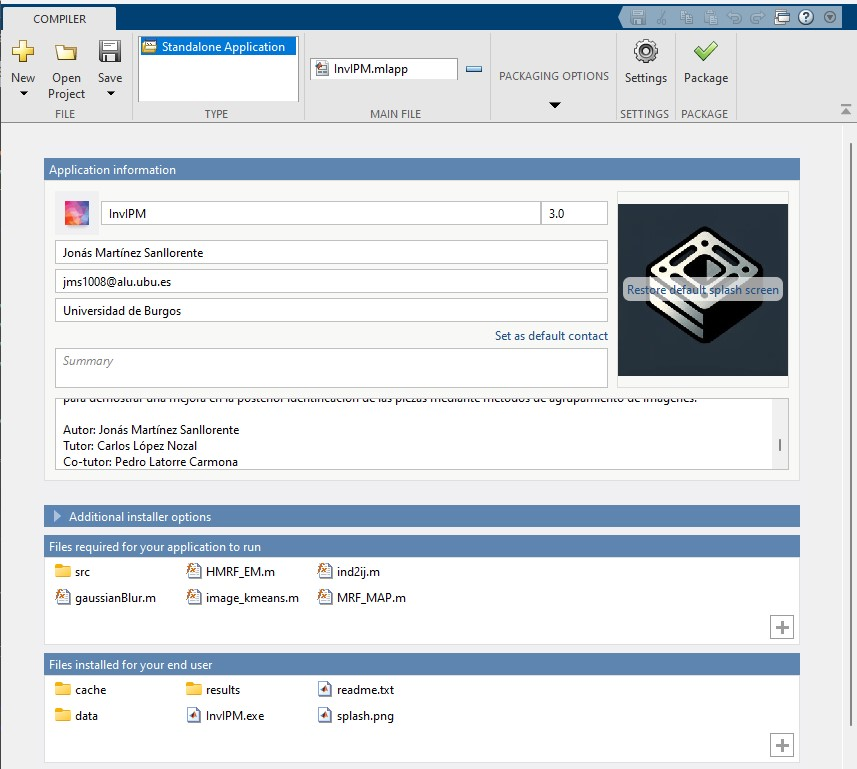
\includegraphics[scale=0.4]{standalone_app}
  \caption{Creación de MATLAB Standalone App.}
  \label{fig:standalone_app}
\end{figure}

\subsubsection{Ejecución de la Standalone App}\label{ejecución-de-la-standalone-app}

Al abrir el archivo `InvIPM.exe', se accederá a la aplicación, la cual ejecutará todos los scripts y el código de manera transparente para el usuario, mostrando únicamente los directorios deseados. En mi caso, estos serían:

\begin{itemize}
    \item El directorio `/data' ya que contienen las imágenes de prueba con sus respectivas imágenes ground truth.
    \item El directorio `/cache' ya que sera donde se almacenen todos los resultados de antiguas ejecuciones de forma temporal.
    \item El directorio `/results' ya que sera la ruta por defecto que se le ofrezca al usuario cuando este desee guardar los resultados de una ejecución.
    \item El README con las pertinentes explicaciones.
    \item El splash de la aplicación.
\end{itemize}

\section{Pruebas del sistema}\label{pruebas-del-sistema}

\subsection{Casos de prueba}\label{casos-de-prueba}

Se han creado múltiples tests unitarios para comprobar el correcto funcionamiento de manera aislada de los scripts que utiliza la aplicación.

Los distintos tests creados son los siguientes:

\begin{itemize}
    \item alvarez\_transformTest.m
    \begin{itemize}
        \item Test básico.
        \item Test de valores extremos.
        \item Test con una imagen uniforme.
        \item Test con una imagen en blanco y negro.
    \end{itemize}
    \item maddern\_transformTest.m
    \begin{itemize}
        \item Test básico.
        \item Test de valores extremos.
        \item Test con una imagen uniforme.
    \end{itemize}
    \item krajnik\_transformTest.m
    \begin{itemize}
        \item Test básico.
        \item Test de valores extremos.
        \item Test con una imagen uniforme.
    \end{itemize}
    \item upcroft\_transformTest.m
    \begin{itemize}
        \item Test básico.
        \item Test de valores extremos.
        \item Test con una imagen uniforme.
    \end{itemize}
    \item calcular\_alphaTest.m
    \begin{itemize}
        \item Test valores básicos.
        \item Test con lambda1 a 0.
        \item Test con las tres lambdas iguales.
    \end{itemize}
    \item calcular\_theta\_krajnikTest.m
    \begin{itemize}
        \item Test valores básicos.
        \item Test con una imagen uniforme.
        \item Test con una imagen en blanco y negro.
    \end{itemize}
    \item calcular\_coincidenciaTest.m
    \begin{itemize}
        \item Test con imágenes iguales.
        \item Test con imágenes diferentes.
    \end{itemize}
    \item check\_cacheTest.m
    \begin{itemize}
        \item Test existe caché (la crea, añade una imagen y luego borra la caché).
    \end{itemize}
    \item convertir\_a\_blanco\_negro\_con\_bordesTest.m
    \begin{itemize}
        \item Test con un caso perfecto.
        \item Test con un caso no perfecto.
    \end{itemize}
    \item imagen\_tres\_canalesTest.m
    \begin{itemize}
        \item Test con una imagen de cuatro canales.
        \item Test con una imagen de tres canales.
    \end{itemize}
    \item metodos\_agrupamientoTest.m
    \begin{itemize}
        \item Test de K-Means sin imagen ground truth.
        \item Test de K-Means con imagen ground truth.
    \end{itemize}
    \item metodos\_invariantesTest.m
    \begin{itemize}
        \item Test de el invariante de Álvarez.
        \item Test de el invariante de Maddern.
    \end{itemize}
    \item moda\_colorTest.m
    \begin{itemize}
        \item Test básico, un color aparece repetido.
        \item Test de colores únicos.
    \end{itemize}
    \item segmentar\_imagen\_fuzzy\_CMeansTest.m
    \begin{itemize}
        \item Test básico.
    \end{itemize}
    \item segmentar\_imagen\_GMMTest.m
    \begin{itemize}
        \item Test básico.
    \end{itemize}
    \item segmentar\_imagen\_KMeansTest.m
    \begin{itemize}
        \item Test básico.
    \end{itemize}
\end{itemize}

Como se puede apreciar, ni PCA ni HMRF\_EM tienen test unitarios propios ya que dichas librerías ya han sido testeadas por sus desarrolladores.

\subsection{Ejecución de los casos de prueba}\label{ejecución-de-los-casos-de-prueba}

Para ejecutar los casos de prueba, como viene indicado en el README de la carpeta test, hemos de copiar los scripts del directorio `/test' al directorio `/functions'.

Una ver realizado esto tenemos dos opciones.
\begin{enumerate}
    \item \textbf{Ejecutar uno a uno:} si deseas ejecutar un test específico por separado, abre la consola de comandos y utiliza el siguiente comando, reemplazando `nombreDelTest' por el nombre del test que deseas ejecutar `disp(runtests(`nombreDelTest'))'.
    \item \textbf{Ejecutar todos a la vez:} si lo que quieres es ejecutar todos a la vez, simplemente tienes que ejecutar el archivo `run\_all\_tests.m'. Este archivo se encargará de correr todos los tests de forma automática.
    
    Los resultados de ejecutar todos los tests son los que se pueden observar en la figura \ref{fig:resultados_tests}.
\end{enumerate}

\imagen{resultados_tests}{Resultados de la ejecución de los tests.}
\apendice{Documentación de usuario}

\section{Introducción}\label{introducción-manual-usuario}

Este apéndice está destinado a abordar los temas relacionados con la parte del usuario. Aquí se tratarán los requisitos, la instalación de la aplicación y el manual de uso para el usuario.

\section{Requisitos de usuarios}\label{requisitos-de-usuario}

Los requisitos necesarios para poder utilizar la aplicación son:

\begin{itemize}
    \item Disponer de un ordenador, ya que se trata de una aplicación de escritorio.
    \item MATLAB Runtime 2023b, disponible en \url{https://es.mathworks.com/products/compiler/matlab-runtime.html}.
\end{itemize}

\subsection{MATLAB Runtime 2023b}\label{matlab-2023b-usuario}

El único programa necesario para la ejecución de este proyecto es MATLAB Runtime, específicamente la versión correspondiente a MATLAB 2023b. Para descargarlo, debes ir a la página oficial de MathWorks \cite{matlabRuntime}. Una vez descargado e instalado, no se requiere una cuenta de MATLAB para su uso. MATLAB Runtime permite ejecutar aplicaciones compiladas con MATLAB Compiler sin necesidad de tener una licencia de MATLAB completa.

\section{Instalación}\label{instalación-usuario}

No hay un proceso de instalación adicional aparte de las dependencias mencionadas anteriormente, ya que la aplicación es auto contenida. Esto significa que todos los archivos y bibliotecas necesarios ya están incluidos en la carpeta de la versión. Gracias a esto, la instalación y el uso se simplifican considerablemente, permitiendo que incluso los usuarios sin experiencia en MATLAB tengan una experiencia agradable.

El primer paso será ir al repositorio de GitHub y descargarse la ultima release, esto se puede hacer tal y como se muestra en la figura \ref{fig:app_release} en el menú de la derecha:

\imagen{app_release}{Instalación de la release desde GitHub.}

La figura \ref{fig:app_release} muestra una la release v0.3.1 de la aplicación InvIPM en GitHub incluyendo la versión, una breve descripción de los cambios y funcionalidades nuevas respecto a la anterior y un zip con los binarios para ejecutar en Linux y en Windows. En este apartado es muy importante descargarse la versión correspondiente al sistema operativo utilizado.

Una vez descargado el archivo zip tendremos que descomprimirlo. Tras ello, nos quedaran una serie de archivos y carpetas en el directorio deseado. Estas son:
    \begin{itemize}
        \item /InvIPM.exe: este es el ejecutable de la aplicación.
        \item /readme.txt: es un documento de ayuda el cual nos indica los requisitos necesarios además de como ejecutar la aplicación.
        \item /data: en este directorio se almacenan las imágenes de ejemplo que trae la propia aplicación, estas podrán ser borradas por el usuario si así lo desea.
        \item /cache: en este directorio se almacenaran las imágenes guardadas en caché.
        \item /results: este es el directorio que se le ofrece al usuario por defecto cuando quiere guardar los resultados de una ejecución.
        \item /splash.png: es la imagen que aparece nada mas abrir la aplicación.
    \end{itemize}
    
\section{Manual del usuario}\label{manual-del-usuario}

Sección dedicada a la redacción de un manual sencillo para que el usuario comprenda cómo utilizar la aplicación.

\subsection{Bienvenida}\label{bienvenida}

Nada más entrar en la aplicación, se presentará una imagen de bienvenida que explica en términos generales el objetivo de la misma, además de mostrar el autor y los tutores del proyecto. El contenido de esta pantalla se muestra en la figura \ref{fig:app_bienvenida}

\imagen{app_bienvenida}{Apartado de bienvenida de InvIMP.}

En la figura \ref{fig:app_bienvenida} se puede apreciar el aspecto de la ventana de bienvenida de InvIPM.

En la parte superior derecha de esta pantalla, se encuentra un selector de idioma entre español e inglés, con sus correspondientes banderas. Esto lo hace más autoexplicativo, permitiendo al usuario identificarlo sin necesidad de leer el texto. Esto es especialmente útil cuando la aplicación está en un idioma diferente al del usuario.

\subsection{Exploración de algoritmos}\label{exploración-de-algoritmos}

En este apartado, es donde el usuario puede cargar, ejecutar y visualizar los resultados de la ejecución.

\imagen{app_exploracion}{Apartado de exploración de algoritmos de InvIMP.}

En la figura \ref{fig:app_exploracion} se puede apreciar el aspecto de la ventana de exploración de algoritmos de InvIPM.

\subsubsection{Selección de imagen}\label{selección-de-imagen}

Mediante el botón de `Cargar imagen de pieza metálica', se podrá seleccionar una imagen proporcionada por el sistema o una propia sobre la cual se aplicarán los algoritmos más adelante.

\subsubsection{Selección de imagen ground truth}\label{selección-de-imagen-ground-truth}

En caso de no ser una imagen proporcionada por el sistema se habilitará el botón de `Cargar imagen ground truth (opcional)' para de esta manera poder proporcionar una propia. Esta imagen como indica el texto no es necesaria para la ejecución exceptuando el obtener el porcentaje de acierto.

\subsubsection{Selección de algoritmo invariante}\label{selección-de-algoritmo-invariante}

Se proporcionan los distintos métodos invariantes:

\begin{itemize}
    \item Álvarez.
    \item Maddern.
    \item Krajnık.
    \item Upcroft.
    \item PCA.
\end{itemize}

Estos están ordenados de manera que el primero es el que mejores resultados ofrece según las pruebas realizadas. Por otro lado, PCA, aunque muestra una clara mejoría en muchas situaciones, es un enfoque más clásico que numéricamente no alcanza resultados tan buenos como otros métodos, en concreto Álvarez.

\subsubsection{Selección de algoritmo de agrupamiento}\label{selección-de-algoritmo-de-agrupamiento}

Se proporcionan los distintos métodos de agrupamiento:

\begin{itemize}
    \item K-Means.
    \item Fuzzy C-Means.
    \item Gaussian Mixtures.
    \item Información espacial, el cual es HMRF\_EM.
\end{itemize}

Estos están ordenados de manera que el primero es el menos costoso computacionalmente, por lo que ofrecerá mejores tiempos de ejecución. El último, en cambio, tiene tiempos de ejecución más largos, ya que es un algoritmo que no solo considera el color de un píxel en particular, sino también el de los píxeles circundantes.

\subsubsection{Selección de número de centros}\label{selección-de-número-de-centros}

Mediante este cuadro de texto el usuario puede indicar el número de centros a utilizar en los algoritmos de agrupamiento. Por defecto este número será 2.

El número de centros ha de cumplir las siguientes condiciones:

\begin{itemize}
    \item Ser un numero positivo.
    \item Ser igual o mayor que 2.
    \item Ser igual o menor que 10.
\end{itemize}

Esto se debe a que, como mínimo, se necesitan dos centros para poder separar entre pieza y fondo. El máximo se establece porque, a mayor cantidad de centros, aumenta la complejidad computacional, lo cual alargaría considerablemente los tiempos de ejecución.

\subsubsection{Ejecución}\label{ejecución}

Al pulsar el botón de `Ejecutar' se dará inicio a la ejecución sobre la imagen seleccionada de los distintos algoritmos elegidos.Durante la ejecución, se proporcionará retroalimentación sobre el porcentaje de progreso y la etapa que se está calculando en ese momento.

\subsubsection{Representación de resultados}\label{representación-de-resultados}

Tras finalizar la ejecución se mostraran en la parte derecha cuatro imágenes, estas serán:

\begin{itemize}
    \item La imagen original (arriba a la izquierda).
    \item La imagen original segmentada (arriba a la derecha).
    \item La imagen invariante (abajo a la izquierda).
    \item La imagen invariante segmentada (abajo a la derecha).
\end{itemize}

En el caso de que se haya utilizado una imagen proporcionada por la aplicación o que el usuario haya proporcionado una imagen de referencia (ground truth), el título tanto de la imagen original segmentada como de la imagen invariante segmentada mostrará el porcentaje de acierto. De esta manera, el usuario podrá comparar los resultados no solo visualmente, sino también numéricamente.

\subsection{Histórico de exploraciones}\label{histórico-de-exploraciones}

En este apartado, se presenta una tabla en la cual aparecen, a modo de lista, todas las ejecuciones realizadas tanto en esta sesión como en sesiones previas. El contenido de las columnas de esta tabla es el siguiente:

\begin{itemize}
    \item \textbf{Nombre del fichero:} este es el nombre del archivo que el usuario seleccionó.
    \item \textbf{Fecha:} esta es la fecha de la ejecución. Esta está en formato DD-MMM-YYY HH-MM-SS.
    \item \textbf{Algoritmo invariante:} muestra el nombre del algoritmo invariante aplicado sobre la imagen. En el caso de no haberse aplicado ningún algoritmo invariante muestra `No aplicado'.
    \item \textbf{Algoritmo de agrupamiento:} muestra el nombre del algoritmo de agrupamiento aplicado sobre la imagen. En el caso de no haberse aplicado ningún algoritmo de agrupamiento muestra `No aplicado'.
    \item \textbf{Número de centros:} muestra la cantidad de centros utilizados en el algoritmo de agrupamiento aplicado sobre la imagen. En el caso de no haberse aplicado ningún algoritmo de agrupamiento muestra `-'.
    \item \textbf{Imagen ground truth:} indica mediante `Sí' o `No' el si la ejecución de dicha imagen tenia o bien imagen asociada o el usuario había proporcionado una propia.
    \item \textbf{Medida de calidad:} indica la tasa de acierto que se ha logrado al comparar la imagen correspondiente a dicha fila con si imagen ground truth. En caso de no tener imagen ground truth esta celda estará en blanco.
    \item \textbf{Archivo:} muestra un checkbox el cual al pulsar sobre el abre en una nueva ventana la imagen correspondiente a dicha fila. Esta nueva ventana tiene una serie de opciones aparte de la visualización permitiendo que el usuario la guarde o imprima entre otras opciones.
\end{itemize}

El usuario también puede si lo desea ordenar la tabla por la columna que quiera.

\imagen{app_historico}{Apartado de histórico de exploraciones de InvIMP.}

En la figura \ref{fig:app_historico} se puede apreciar el aspecto de la ventana de histórico de exploraciones de InvIPM.

A parte de la tabla, en la parte inferior hay dos botones, uno para ver las imágenes y otro para borrar el contenido de la memoria cache. 

\subsubsection{Ver imágenes}\label{ver-imágenes}

Al pulsar en este botón se abrirá una ventana nueva donde se podrá ver y seleccionar todas aquellas imágenes que están almacenadas en la memoria caché.

\subsubsection{Borrar datos}\label{borrar-datos}

Al pulsar este botón, aparecerá una ventana emergente indicando si realmente se desea borrar de forma irreversible el contenido de la memoria caché. En caso de pulsar el botón `Borrar', se eliminará su contenido y se actualizará la tabla, ya que dichas imágenes no se encontrarán disponibles. Tras esto, se indicará que la memoria caché se ha borrado exitosamente.

\subsection{Ayuda}\label{ayuda}

En este apartado, tal y como se muestra en la figura \ref{fig:app_ayuda}, se puede obtener información sobre el funcionamiento, los algoritmos invariantes, los algoritmos de agrupamiento, la caché y la tasa de acierto. Al estar la propia documentación implementada dentro de la aplicación, resulta muy cómodo buscar información sobre cualquier tema de interés. 

Además, el idioma de la documentación corresponde con el que se ha seleccionado en la bienvenida.

\imagen{app_ayuda}{Apartado de ayuda de InvIMP.}

En la figura \ref{fig:app_ayuda} se puede apreciar el aspecto de la ventana de ayuda de InvIPM.
\apendice{Anexo de sostenibilización curricular}

\section{Introducción}
Este anexo incluirá una reflexión personal del alumnado sobre los aspectos de la sostenibilidad que se abordan en el trabajo.
Se pueden incluir tantas subsecciones como sean necesarias con la intención de explicar las competencias de sostenibilidad adquiridas durante el alumnado y aplicadas al Trabajo de Fin de Grado.

Más información en el documento de la CRUE \url{https://www.crue.org/wp-content/uploads/2020/02/Directrices_Sosteniblidad_Crue2012.pdf}.

Este anexo tendrá una extensión comprendida entre 600 y 800 palabras.



\bibliographystyle{plain}
\bibliography{bibliografiaAnexos}

\end{document}
